\documentclass[11pt]{article}
\usepackage[a4paper,margin=2.2cm]{geometry}
\usepackage{amsmath,amssymb}
\usepackage{graphicx}
\usepackage{booktabs}
\usepackage{array}
\usepackage{float}
\usepackage{listings}
\usepackage[hidelinks]{hyperref}
\graphicspath{{figures/}}
\lstset{basicstyle=\ttfamily\footnotesize, breaklines=true, columns=fullflexible, frame=single, showstringspaces=false}
\setlength{\parskip}{0.5em}
\setlength{\parindent}{0pt}

\title{When does the LayerNorm Jacobian kink reach a controller?\\[0.3em]
\large Companion notes to the presentation, slides 1 to 14 (setup, kink, LQR): setup, reproducibility and figure explanations}
\author{Binoy George}
\date{28 October 2026}

\begin{document}
\maketitle
{\setlength{\parskip}{0pt}\tableofcontents}
\newpage

%=====================================================================
\section{How to relate to the slides}

Slide numbers in this document are the numbers printed on the powerpoint slides. Sections map to slides as follows.

\begin{center}
\footnotesize
\setlength{\tabcolsep}{4pt}
\begin{tabular}{lllll}
\toprule
Printed & Position in file & Topic & Figure & Here \\
\midrule
\multicolumn{5}{l}{Part 1} \\
1 & 1 & Cover & -- & -- \\
-- & 2--3 & Glossary (unnumbered) & -- & -- \\
2--3 & 4--5 & Question, setup & f02 & Sections \ref{sec:question} to \ref{sec:eval}, Figures \ref{fig:data}, \ref{fig:arch} \\
4 & 6 & Why the early analysis was hard & f03 & Section \ref{sec:s2}, Figure \ref{fig:slice} \\
5 & 7 & Kink maps (2-D) & f05 & Section \ref{sec:s3}, Figure \ref{fig:zoom} \\
6 & 8 & The kink as crests and troughs (3-D) & f16 & Section \ref{sec:s3}, Figure \ref{fig:surf3d} \\
7 & 9 & Closed form and petals & f06 & Sections \ref{sec:kink}, \ref{sec:s3}, Figure \ref{fig:petals} \\
8 & 10 & Fixed LQR & f07 & Section \ref{sec:s4}, Figures \ref{fig:four}, \ref{fig:timeline} \\
9--10 & 11--12 & Rescheduled LQR; path-colour test & f09, f10 & Section \ref{sec:s5}, Figures \ref{fig:resched}, \ref{fig:pathcolour} \\
11--12 & 13--14 & Failure vs setpoint; setpoint law & f11, f12 & Section \ref{sec:s6}, Figures \ref{fig:setpoint}, \ref{fig:law} \\
13--14 & 15--16 & Swap test example; which slope & f13, f15 & Section \ref{sec:s7}, Figures \ref{fig:swap9} to \ref{fig:swaprates} \\
\midrule
\multicolumn{5}{l}{Part 2} \\
15 & 17 & From LQR to DPC & -- & DPC settings, Section \ref{sec:dpcctrl} \\
16 & 18 & DPC: what failure looks like & -- & DPC settings, Section \ref{sec:dpcctrl} \\
17 & 19 & Why: the gradient explodes & -- & DPC settings, Section \ref{sec:dpcctrl} \\
18 & 20 & No barrier: a chaotic gradient & -- & DPC settings, Section \ref{sec:dpcctrl} \\
19 & 21 & Warm start at the good controller & -- & DPC settings, Section \ref{sec:dpcctrl} \\
20 & 22 & DPC swap test & -- & DPC settings, Section \ref{sec:dpcctrl} \\
21 & 23 & Scorecard & -- & DPC settings, Section \ref{sec:dpcctrl} \\
22 & 24 & Synthesis & -- & DPC settings, Section \ref{sec:dpcctrl} \\
23 & 25 & Limits and next steps & -- & Not covered \\
24 & 26 & Takeaway & -- & Not covered \\
\midrule
\multicolumn{5}{l}{Appendix} \\
A1 & 27 & Animation of the four LQR cases & f07 & Section \ref{sec:s4}, Figure \ref{fig:four} \\
A2 & 28 & Animation: how DPC controllers fail & -- & Not covered \\
A3 & 29 & Animation: the warm start is expelled & -- & Not covered \\
A4--A7 & 30--33 & Backups for Part 1 & f01, f04, f08, f14 & Figures \ref{fig:data}, \ref{fig:fullbox}, \ref{fig:timeline}, \ref{fig:swap8} \\
A8 & 34 & Warm start in the phase plane & -- & Not covered \\
\bottomrule
\end{tabular}
\end{center}

Notation. $x$ is the state, $u$ the input, $z=(x,u)$. The true plant has slopes $A=\partial f/\partial x$ and $B=\partial f/\partial u$. The surrogate is $\hat F(x,u)$ with slopes $\hat J_x=\partial \hat F/\partial x$ and $\hat J_u=\partial \hat F/\partial u$. When a controller reads the surrogate's slopes at one point we write them $\hat A$ and $\hat B$. A seed is written $s\in\{0,\dots,9\}$.

%=====================================================================
\section{The question (slides 2 to 3)}\label{sec:question}

A neural network trained on one-step transitions can predict the next state very accurately on average and still have badly wrong derivatives in a small region. Controllers built from a model use its derivatives: a linearised design (LQR) uses them at an operating point, gain scheduling uses them along the trajectory, and differentiable predictive control (DPC) backpropagates through them over a long horizon. The question of the study is:

Does the derivative defect created by pre-norm LayerNorm (the kink) reach the controllers designed from an accurate surrogate, and if so through which mechanism?

The hypothesis that people implicitly assume, called H0 here, is that a surrogate with small prediction error gives controllers close to those designed from the true plant. Slides 2 to 14 test H0 for two linear-quadratic controllers; slides 15 to 22 do the same for DPC. The answer is no: with LayerNorm surrogates of the same prediction accuracy as kink-free ones, the fixed LQR fails on 26.5 percent of runs (10.8 percent catastrophically) against 0.6 percent (0 percent) for a static-norm surrogate. The rest of the first half of the slides locates where, why and through which slope this happens.

%=====================================================================
\section{The plant}\label{sec:plant}

The plant is scalar, linear and open-loop unstable:
\begin{equation}
x_{k+1} = f(x_k,u_k) = A x_k + B u_k, \qquad A = 1.03,\quad B = 0.01 .
\end{equation}
The input is limited to $|u|\le 10$ (the actuator range and the range of the training data). The input that holds a setpoint $r$ is
\begin{equation}
u_{ss}(r) = \frac{(1-A)\,r}{B} = -3r ,
\end{equation}
so the true equilibria form the line $u=-3x$ (dotted in many figures). With $|u|\le 10$ the plant can hold setpoints up to $|r|\le 3.33$ and can be steered to the origin from $|x_0|<3.33$.

Why this plant. It is the simplest plant on which the kink can be traced from the network weights to a control failure step by step: the true slopes are constants, the LQR gain has a closed form, and the kink location has a closed form (Section~\ref{sec:kink}). Two features make it a stress test. First, $A>1$: the stability margin is $A-1=0.03$, so a small error in $\hat A$ is large compared with the margin. Second, the control authority $B=0.01$ is low: the controller needs inputs about 100 times the state error (the true LQR gain is $K=10.29$), and the effect of $u$ on the output is small (at most $\pm 0.1$ over the data range, against $\pm 4.1$ for the effect of $x$), so the $u$-slope is the hardest thing for the network to learn and every error in it is measured relative to a small number.

The code (level1\_core.py) also contains a weakly nonlinear version (parameter eps\_nl); all results here use the linear plant, eps\_nl = 0.

%=====================================================================
\section{The data sets}\label{sec:data}

\subsection{Training data}
For each seed $s$ one training set of $n=20\,000$ transitions is drawn:
\begin{equation}
x_i \sim \mathcal U[-4,4],\quad u_i \sim \mathcal U[-10,10],\quad y_i = A x_i + B u_i + \sigma \varepsilon_i,\quad \varepsilon_i\sim\mathcal N(0,1),\quad \sigma = 0.01,
\end{equation}
independently, with the NumPy generator \texttt{default\_rng(1000 + s)}. So every seed has its own data set, and every surrogate family trained for seed $s$ sees exactly the same data. The inputs fill the box $[-4,4]\times[-10,10]$ uniformly (Figure~\ref{fig:data}). The sample standard deviations are $s_x=2.31$, $s_u=5.78$ and $\mathrm{Var}(y)=5.65$. The noise level $\sigma=0.01$ equals the change in $y$ caused by one unit of $u$.

\subsection{Test data}
A noiseless test set of 4000 transitions from the same box, generator seed 12345, is the same for every seed and every family. It is used only to report the relative test error
\begin{equation}
\text{rel-MSE} = \frac{\frac{1}{n}\sum_i (\hat F(x_i,u_i)-f(x_i,u_i))^2}{\mathrm{Var}(y)} .
\end{equation}

\subsection{Slope labels (only for the two slope-trained families)}\label{sec:labels}
Two families add a Jacobian loss. Its labels are not the true slopes: they are estimated from the same 20\,000 noisy transitions, so no information beyond the data is used. For every training input a local quadratic surface is fitted by weighted least squares to its $k$ nearest neighbours (distance measured after dividing $x$ and $u$ by their standard deviations), with Epanechnikov weights $1-t^2$, $t=d/d_{(k)}$; the fitted linear coefficients are the labels $\hat J_x^{\text{lab}},\hat J_u^{\text{lab}}$. The neighbour count $k$ is chosen from $\{40,80,160,320,640,1280\}$ by minimising an estimate of label bias squared plus variance (a doubling trick comparing $k$ and $2k$, with the noise variance estimated from residuals). For seeds 0 and 9 this gives $k=1280$, estimated noise $\hat\sigma=0.0100$, and label errors of 1.5 to 1.9 percent (median) and 4 to 6 percent (90th percentile) for $\hat J_u^{\text{lab}}/B$, and $5\times10^{-4}$ (median) for $\hat J_x^{\text{lab}}$. Labels are computed once per seed and cached (files labels\_seed$s$\_sigma0.01\_epan.npz).

Correction to the presentation briefing: two-stage training uses these estimated labels, not the true slopes.

\subsection{Evaluation grids used up to slide 14}\label{sec:grids}
\begin{itemize}
\item Setpoints: $r\in\{-2,-1,-0.5,-0.25,-0.1,0,0.1,0.25,0.5,1,2\}$ (11 values).
\item Starts: $x_0\in\{-3,-2.25,-1.5,-0.75,0,0.75,1.5,2.25,3\}$ (9 values, linspace(-3, 3, 9)).
\item Seeds: 0 to 9. This gives $11\times 9\times 10=990$ runs per surrogate family and controller. Pairs with $|x_0-r|<0.5$ are excluded from all rates because the reference cost there is tiny and any small offset gives a huge relative gap; 11 of the 99 pairs are excluded, leaving 88 per seed and 880 per family and controller.
\item Map grids for the figures: regular grids over the box or a zoom window (resolution stated in each caption), evaluated with automatic differentiation of the network.
\end{itemize}

\begin{figure}[H]
\centering
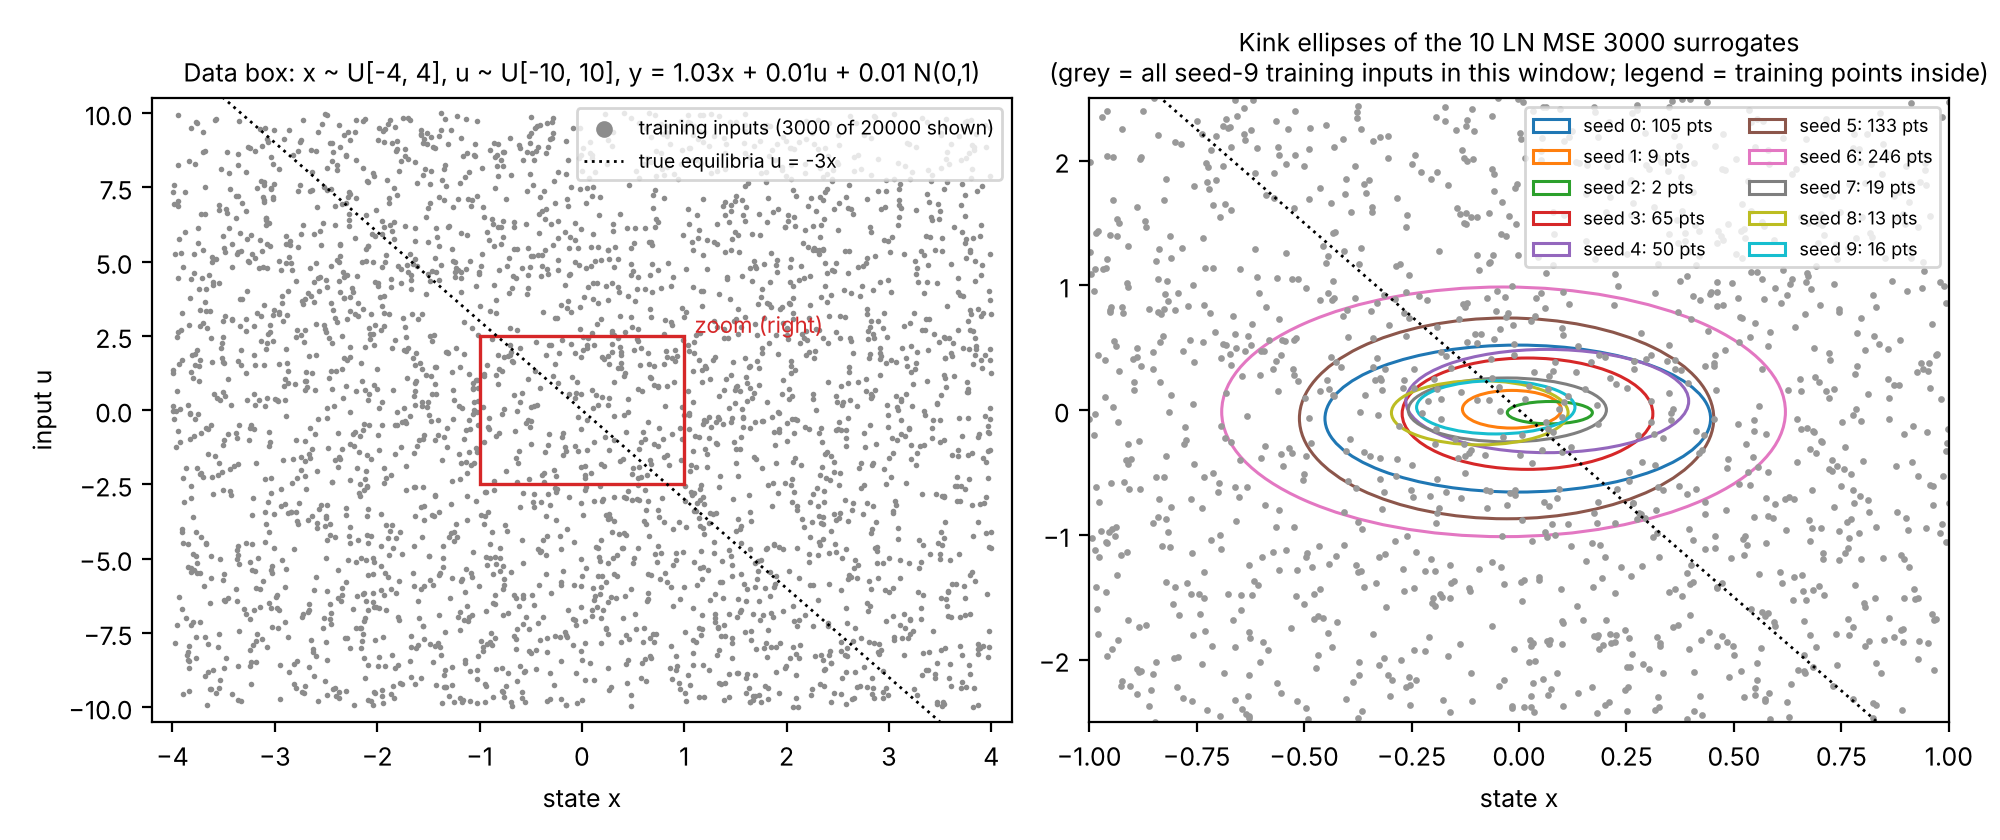
\includegraphics[width=\textwidth]{f01_data_and_kinks.png}
\caption{Left: the training inputs of seed 9 (3000 of the 20\,000 shown) fill the box uniformly; dotted line = true equilibria $u=-3x$; the red rectangle is the zoom shown on the right. Right: the closed-form kink ellipses (Section~\ref{sec:kink}) of the ten LayerNorm MSE 3000 surrogates, all centred within 0.1 of the origin, with the number of that seed's training points that fall inside each ellipse. The narrow kinks of seeds 1, 2, 8 and 9 contain 2 to 16 of the 20\,000 training points (0.01 to 0.08 percent), so a value loss barely sees them. Grey points are seed 9's inputs in the window.}
\label{fig:data}
\end{figure}

%=====================================================================
\section{The surrogate network}\label{sec:net}

\subsection{Architecture}
Every surrogate has the same pre-norm residual architecture (function F\_point in level1\_core.py), with encoder width $H=16$ and branch width 32:
\begin{align}
h &= Ez + b \in\mathbb R^{16}, \qquad z=(x,u)^\top,\ E=[\,e_x\ \ e_u\,]\in\mathbb R^{16\times 2},\\
v &= \mathrm{N}(h) \quad\text{(normalisation, three variants below)},\\
g &= G(\gamma\odot v+\beta),\qquad G(y) = W_2^\top\,\mathrm{GELU}\!\big(W_1^\top y+b_1\big) + b_2 \in\mathbb R^{16},\\
\hat F(x,u) &= w_d^\top (h + g) + b_d .
\end{align}
Here $W_1\in\mathbb R^{16\times 32}$, $W_2\in\mathbb R^{32\times 16}$, and GELU is the exact (erf) version. The skip path carries $h$ past the branch, so the output is a linear function of $(x,u)$, namely $w_d^\top(Ez+b)+b_d$, plus the branch term $w_d^\top g$. The code stores $E$ transposed, as a $2\times16$ array p[``E''] (the reference derivation warns about the same point). In the reference's notation $v$ is $\hat h$ and $w_d^\top$ is $W_d$. The normalisation variants are
\begin{align}
\text{LayerNorm:}&\quad \mathrm N(h) = \frac{h-\bar h\mathbf 1}{\sqrt{\frac1H\|h-\bar h\mathbf 1\|^2+\epsilon}},\qquad \epsilon=10^{-6},\\
\text{static norm:}&\quad \mathrm N(h) = \frac{h-\bar h\mathbf 1}{s_0},\\
\text{no norm:}&\quad \mathrm N(h) = h .
\end{align}
Here $\bar h$ is the mean of the 16 entries of $h$, and $s_0$ is the LayerNorm scale at initialisation averaged over the training inputs (one number per seed, frozen). Static norm keeps the centring and a fixed scale but removes the data-dependent division, which is what creates the kink; no norm removes both. They are the two kink-free controls. In all three variants the branch receives $\gamma\odot v+\beta$; in the no-norm case $\gamma$ and $\beta$ act directly on $h$, where they add nothing a network cannot already represent, since $W_1^\top(\gamma\odot h+\beta)+b_1 = (W_1^\top\mathrm{diag}(\gamma))h + (W_1^\top\beta+b_1)$. All three variants have the same 1169 parameters.

\begin{figure}[H]
\centering
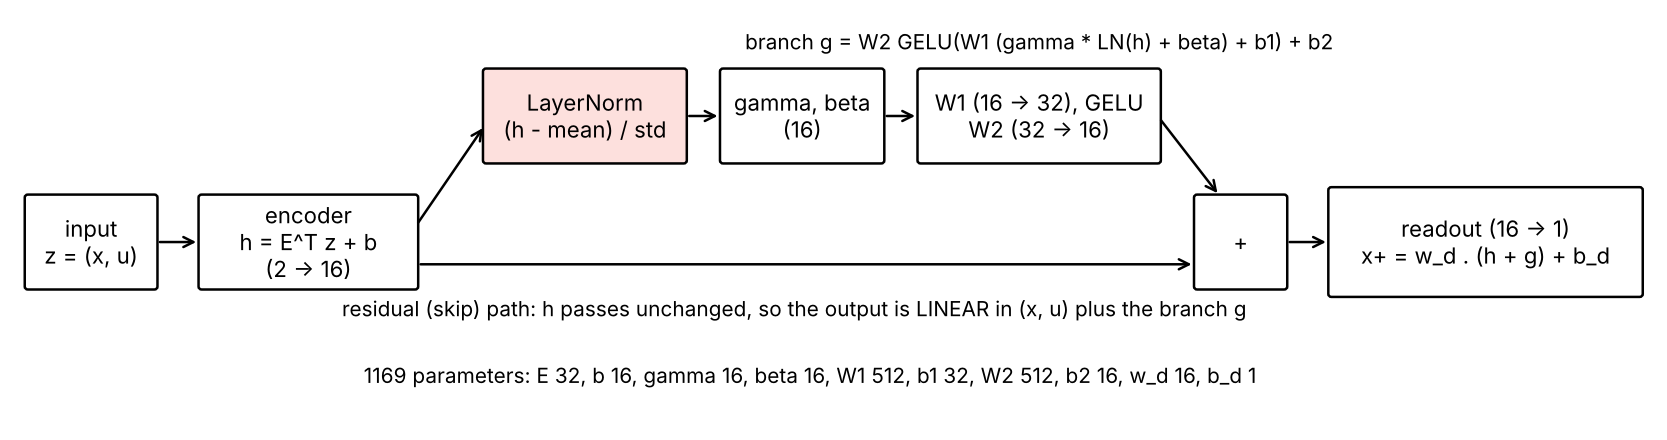
\includegraphics[width=\textwidth]{f02_architecture.png}
\caption{The surrogate. The LayerNorm block (shaded) is the only difference between the LayerNorm, static-norm and no-norm surrogates.}
\label{fig:arch}
\end{figure}

\subsection{Parameters and initialisation}
\begin{center}
\begin{tabular}{lrl}
\toprule
Parameter & Count & Initialisation \\
\midrule
$E$ (encoder) & 32 & Glorot uniform \\
$b$ (encoder bias) & 16 & zeros \\
$\gamma$, $\beta$ (norm gain and shift) & 16 + 16 & ones, zeros \\
$W_1$, $b_1$ & 512 + 32 & Glorot uniform, zeros \\
$W_2$, $b_2$ & 512 + 16 & Glorot uniform, zeros \\
$w_d$, $b_d$ (readout) & 16 + 1 & Glorot uniform, zero \\
\midrule
Total & 1169 & key jax.random.PRNGKey($s$) \\
\bottomrule
\end{tabular}
\end{center}
All arithmetic for the surrogates is in float64. The encoder bias starts at zero; Section~\ref{sec:kink} explains why this places every kink near the origin.

%=====================================================================
\section{Training: the six surrogate families}\label{sec:train}

\subsection{Losses}
The value loss is the full-batch mean squared error
\begin{equation}
\mathcal L_{\text{MSE}} = \frac1n\sum_{i=1}^n\big(\hat F(x_i,u_i)-y_i\big)^2 .
\end{equation}
The slope loss adds, at every step, a Jacobian penalty on $M=2048$ points drawn uniformly with replacement from the training inputs (a fresh draw each step, random key 10000 + $s$):
\begin{equation}
\mathcal L_{\text{slope}} = \mathcal L_{\text{MSE}} + \lambda\,\frac1M\sum_{j=1}^M\Big[s_x^2\big(\hat J_x(z_j)-\hat J_x^{\text{lab}}(z_j)\big)^2 + s_u^2\big(\hat J_u(z_j)-\hat J_u^{\text{lab}}(z_j)\big)^2\Big],\qquad \lambda = 1 .
\end{equation}
The factors $s_x^2$, $s_u^2$ make the penalty invariant to the units of $x$ and $u$. The surrogate's slopes inside the loss are computed with forward-mode automatic differentiation (jax.jvp).

\subsection{Optimiser}
Adam with learning rate $3\times10^{-3}$, $\beta_1=0.9$, $\beta_2=0.999$, $\epsilon_{\text{Adam}}=10^{-8}$, no weight decay, full batch (one step = one epoch). At a switch between training phases the Adam moments and step counter are reset. The ten seeds of one family are trained together (vectorised with jax.vmap), each with its own data, initialisation and random draws.

\subsection{The six families}
\begin{center}
\begin{tabular}{lll}
\toprule
Family (name in the slides) & Normalisation & Training schedule \\
\midrule
LN MSE 3000 & LayerNorm & 3000 steps of $\mathcal L_{\text{MSE}}$ \\
LN MSE 12000 & LayerNorm & 12\,000 steps of $\mathcal L_{\text{MSE}}$ \\
LN slope from step 0 & LayerNorm & 3000 steps of $\mathcal L_{\text{slope}}$ (estimated labels) \\
LN two-stage & LayerNorm & 3000 steps of $\mathcal L_{\text{MSE}}$, then 1000 steps of $\mathcal L_{\text{slope}}$ \\
no norm & none & 3000 steps of $\mathcal L_{\text{MSE}}$ \\
static norm & static & 3000 steps of $\mathcal L_{\text{MSE}}$ \\
\bottomrule
\end{tabular}
\end{center}
In the code these are the configurations ``MSE (3000)'', ``MSE (12000)'', ``J\_x + J\_u (3000)'', ``J\_x + J\_u (two-stage)'', ``no norm, MSE'' and ``static norm, MSE'' (level1\_configs in level1\_core.py and surrogate\_configs in dpc\_core.py).

\subsection{Accuracy reached}
All families reach relative test errors between $10^{-8}$ and $5\times10^{-5}$, most seeds between $10^{-7}$ and $3\times10^{-6}$ (Table~\ref{tab:acc}). For the main family this is a root-mean-square value error of $1\times10^{-3}$ to $4\times10^{-3}$, below the data noise $\sigma=0.01$. Value accuracy does not separate the families; their slopes do. On seed 9 the root-mean-square value error over the whole box is $1.8\times10^{-3}$ for LN MSE 3000 and $2.9\times10^{-3}$ for static norm. The LayerNorm surrogate's value error is not uniformly small: inside its kink it reaches about $0.05$ on seed 9 (Figure~\ref{fig:slice}), but the kink covers well under 0.1 percent of the box, so this hardly changes the averages.

\begin{table}[H]
\centering
\small
\setlength{\tabcolsep}{4pt}
\begin{tabular}{lccc}
\toprule
Family & rel-MSE, range & $\max|\hat J_u/B-1|$: median (range) & $\max|\hat J_x-A|$: median \\
\midrule
LN MSE 3000 & $2.3\times10^{-7}$ -- $3.4\times10^{-6}$ & 18.7 (6.7 -- 200.9) & 0.32 \\
LN MSE 12000 & $1.3\times10^{-8}$ -- $5.4\times10^{-5}$ & 2.8 (0.51 -- 35.5) & 0.025 \\
LN slope from step 0 & $4.9\times10^{-8}$ -- $1.1\times10^{-6}$ & 7.9 (1.6 -- 28.2) & 0.10 \\
LN two-stage & $5.4\times10^{-8}$ -- $1.9\times10^{-5}$ & 1.2 (0.22 -- 3.9) & 0.01 \\
no norm & $1.7\times10^{-7}$ -- $2.7\times10^{-6}$ & 0.77 (0.24 -- 1.2) & 0.02 \\
static norm & $2.4\times10^{-7}$ -- $1.5\times10^{-6}$ & 0.46 (0.15 -- 1.0) & 0.01 \\
\bottomrule
\end{tabular}
\caption{Accuracy of the six families over the ten seeds. Slope errors are the maximum over a $201\times201$ grid of the box plus points on the closed-form kink lines (evaluate\_batch in level1\_core.py). The input slope is reported relative to $B$.}
\label{tab:acc}
\end{table}

%=====================================================================
\section{Seeds and randomness}\label{sec:seeds}

There are ten seeds, $s=0,\dots,9$. One seed index fixes one complete experiment: its data, its network initialisation, its slope-check draws, and (for DPC) its controller initialisation and training starts. All families and controllers use the same seeds, so every comparison between families is paired seed by seed.

\begin{center}
\begin{tabular}{ll}
\toprule
What & Random source \\
\midrule
Training data of seed $s$ & numpy default\_rng(1000 + $s$) \\
Network initialisation & jax PRNGKey($s$) \\
Slope-check point draws (slope families) & jax PRNGKey(10000 + $s$), split every step \\
Test set (all seeds) & numpy default\_rng(12345) \\
Neighbour-count selection for labels & numpy default\_rng(0) \\
DPC controller initialisation (repeat $q$) & PRNGKey(20000 + $s$ + 1000$q$) \\
DPC training starts (repeat $q$) & PRNGKey(30000 + $s$ + 1000$q$) \\
Tracking DPC initialisation / pairs & PRNGKey(50000 + $s$) / PRNGKey(60000 + $s$) \\
\bottomrule
\end{tabular}
\end{center}
The LQR controllers of slides 8 to 14 contain no randomness: given the surrogate they are deterministic.

%=====================================================================
\section{The kink: closed-form geometry}\label{sec:kink}

\subsection{Derivation}
The notation follows the reference derivation of the kink, the September 2026 note ``The Prenorm LayerNorm Jacobian Anomaly''. That note sweeps one input with the other held fixed. The controllers here move in the whole $(x,u)$ plane, so the same steps are written for the two-dimensional input; along the line $u=u^\star$ through the kink centre they reduce exactly to the reference's equations (4.2), (4.5) and (4.6).

The encoder is $h=Ez+b$ with $E\in\mathbb R^{16\times2}$ and columns $e_x$, $e_u$ (Section~\ref{sec:net}). Centring is the orthogonal projector $P=I-\frac1H\mathbf 1\mathbf 1^\top$, so the centred activation is
\begin{equation}
r = Ph = Q_E z + c,\qquad Q_E = PE = [\,q_x\ \ q_u\,]\in\mathbb R^{16\times2},\qquad c = Pb .
\end{equation}
Here $q_x=Pe_x$ is the reference's $q$ for a sweep along $x$, and $q_u=Pe_u$ the one for a sweep along $u$; the reference needs only one such vector because it holds $u$ fixed, and its $c$ then also contains $q_u u$. The matrix is written $Q_E$, after $E$, to keep it apart from the LQR weight $Q$. LayerNorm divides $r$ by its own length,
\begin{equation}
\mathrm{LN}(h) = \frac{r}{\sigma},\qquad \sigma = \sqrt{\frac{\|r\|^2}{H}+\epsilon},
\end{equation}
and because $z$ is two-dimensional, $r$ can only move in a two-dimensional affine subspace of $\mathbb R^{16}$. Its point of closest approach to the origin is
\begin{equation}
z^\star = (x^\star,u^\star) = \arg\min_z\|Q_E z+c\| = -(Q_E^\top Q_E)^{-1}Q_E^\top c,\qquad c_\perp = Q_E z^\star+c,\quad Q_E^\top c_\perp = 0 ,
\end{equation}
the two-dimensional version of the reference's $x^\star=-q^\top c/\|q\|^2$ and $c_\perp$. With the offset $s=z-z^\star$ the cross term vanishes, $r = Q_E s + c_\perp$ and $\|r\|^2 = s^\top Q_E^\top Q_E\,s + \|c_\perp\|^2$, so
\begin{equation}
\mathrm{LN}(h) = \frac{Q_E s + c_\perp}{\sigma(s)},\qquad \sigma(s) = \sqrt{\frac{s^\top Q_E^\top Q_E\,s}{H} + \delta^2},\qquad \delta^2 = \frac{\|c_\perp\|^2}{H} + \epsilon .
\label{eq:ln}
\end{equation}
The denominator is smallest, equal to $\delta$, at $z^\star$, and grows linearly with distance. We write
\begin{equation}
D = \sqrt H\,\delta = \sqrt{\|c_\perp\|^2 + H\epsilon}
\end{equation}
for the kink size; $D$ is the number quoted on the slides and in the tables. The kink is the region where the denominator is still within a factor $\sqrt2$ of its minimum:
\begin{equation}
\mathcal K = \{z:\ s^\top Q_E^\top Q_E\,s \le D^2\},\qquad s = z - z^\star ,
\end{equation}
an ellipse centred at $z^\star$. Its half-widths along the coordinate axes through $z^\star$ are
\begin{equation}
r^*_x = \frac{\delta}{\sqrt{\alpha_x}} = \frac{D}{\|q_x\|},\qquad r^*_u = \frac{\delta}{\sqrt{\alpha_u}} = \frac{D}{\|q_u\|},\qquad \alpha_x = \frac{\|q_x\|^2}{H},\quad \alpha_u = \frac{\|q_u\|^2}{H},
\end{equation}
which is the reference's width $r^\star=\delta/\sqrt\alpha$ (its equation 4.6) for each sweep direction. On the line $u=u^\star$ the offset is $s=(x-x^\star,0)$ and $r = q_x(x-x^\star) + c_\perp$ with $q_x^\top c_\perp=0$, exactly the reference's line (4.4). The half-widths are computed by kink\_center in level1\_core.py. The ellipse drawn in all figures (dashed) and used for the ``kink share'' and the distance $d$ is the axis-aligned ellipse with semi-axes $r^*_x$, $r^*_u$. The exact ellipse $\mathcal K$ is tilted when $q_x^\top q_u\neq0$ (cosine between the columns $-0.39$ to $0.38$ over the ten seeds) but passes through the same four points on the axes.

Inside the kink the normalised features rotate quickly. Differentiating (\ref{eq:ln}) with $\partial r/\partial z = Q_E$ and $\partial\sigma/\partial z = r^\top Q_E/(H\sigma)$,
\begin{equation}
\frac{\partial\,\mathrm{LN}}{\partial z} = \frac{1}{\sigma}\Big(I-\frac{r\,r^\top}{H\sigma^2}\Big)Q_E,\qquad r = Q_E s + c_\perp ,
\end{equation}
which equals $Q_E/\delta$ at the centre, the reference's peak $q/\delta$ (its Section 5.3). The feature gain is inversely proportional to $\delta$, and so to $D$: the narrower the kink, the steeper the features, and the branch passes this steepness to $\hat J_x$ and $\hat J_u$.

What sets $D$. For these surrogates $D=\|c_\perp\|$ to three digits: $D=0.13$ to $0.90$ (Table~\ref{tab:seeds}) while $\sqrt{H\epsilon}=0.004$. This is the reference's geometry-dominated regime (its Section 4.4): the kink width is set by $c_\perp$, the part of the centred encoder bias that the two-dimensional input cannot cancel, and not by $\epsilon$. At initialisation $b=0$, so $c=0$, $z^\star=0$, $c_\perp=0$ and $D=\sqrt{H\epsilon}=0.004$, the reference's $\epsilon$-dominated case: a nearly singular point at the origin. Training moves $b$, which makes $c_\perp$ non-zero and widens the kink, while its centre stays within 0.1 of the origin ($|x^\star|\le0.09$, $|u^\star|\le0.07$). Narrow kinks are seeds whose bias drifted little out of the range of $Q_E$.

Correction to the presentation briefing: changing $\epsilon$ would not change these kinks, because $H\epsilon$ is negligible next to $\|c_\perp\|^2$.

\subsection{Far field: the petals}
Far from the centre ($\rho=\|Q_E s\|\gg D$) expand (\ref{eq:ln}):
\begin{equation}
\mathrm{LN}(h) = \sqrt H\,n + \sqrt H\,\frac{c_\perp}{\rho} + O\!\Big(\frac{D^2}{\rho^2}\Big),\qquad n = \frac{Q_E s}{\rho}.
\end{equation}
The leading term depends only on the direction of $s$. Write that direction as an angle $\theta$ and define the branch output as a function of direction, $\Phi(\theta)=w_d^\top G\big(\gamma\odot\sqrt H n(\theta)+\beta\big)$, with $G$ the branch MLP of Section~\ref{sec:net}. Then the network output and its gradient are
\begin{equation}
\hat F(z) = \underbrace{w_d^\top(Ez+b)+b_d}_{\text{linear}} + \Phi(\theta) + O(1/\rho),\qquad
\nabla\hat F = E^\top w_d + \Phi'(\theta)\,\nabla\theta + O(1/\rho^2),\qquad \|\nabla\theta\|\propto\frac1\rho .
\end{equation}
Three consequences follow.
\begin{enumerate}
\item Moving radially does not change the leading term; moving across directions does, at a rate $\Phi'(\theta)/\rho$. So the slope error away from the kink falls off algebraically with distance (a $1/\rho$ term plus $1/\rho^2$ terms), not exponentially. The kink has long tails. Along any straight line, far from the centre the motion becomes radial, so the derivative along the line decays faster, as $1/\rho^2$: this is the $s^{-2}$ tail of the reference's one-dimensional sweep. The $1/\rho$ term appears in the derivative across the line, for example in $\hat J_u$ at points that lie in the $x$ direction from the centre.
\item $\Phi'(\theta)$ changes sign as $\theta$ goes round, so the error is positive in some directions and negative in others: lobes that alternate around the centre. These are the petals of the heat maps.
\item The value error and the slope error are linked. $\Phi(\theta)$ is bounded and fitted on average, so the value error stays small, while the slope error is its angular derivative divided by the distance. An order-of-magnitude estimate: an angular wiggle of size $a$ in the value gives an input-slope error of about $a/\rho_u$, i.e. a relative error $a/(B\rho_u)$. With $a=10^{-3}$, $B=0.01$ and $\rho_u=0.2$ (a typical kink half-width in $u$) this is already 0.5. The same wiggle gives an $\hat J_x$ error of about $a/\rho_x$, which is small next to $A$ but must be compared with the margin $A-1=0.03$. This is why low control authority makes $\hat J_u$ the vulnerable slope.
\end{enumerate}
What the measurements show (Section~\ref{sec:s3}): the angular sign alternation is clear; along the direction of the setpoints the decay is about $1/d$ (fitted log-log slope $-0.98$ over 440 setpoint designs, with about a decade of scatter); the largest error on a circle decays faster at intermediate distances (slope about $-1.6$ for $\hat J_u$ and $-1.2$ for $\hat J_x$ at $d=2$ to $20$), consistent with the $1/\rho$ term having a small amplitude and the $1/\rho^2$ terms still mattering there. The briefing's ``1/d law'' should therefore be stated as ``algebraic decay, $1/d$ along the setpoint line''.

\subsection{Per-seed geometry of the main family}
\begin{table}[H]
\centering
\footnotesize
\setlength{\tabcolsep}{3pt}
\begin{tabular}{rrrrrrrrrrr}
\toprule
seed & $x^\star$ & $u^\star$ & $r^*_x$ & $r^*_u$ & $D$ & inside & max $|\hat J_u/B-1|$ & max $|\hat J_x-A|$ & fail \% & cat. \% \\
\midrule
0 & $-0.003$ & $-0.068$ & 0.449 & 0.589 & 0.638 & 105 & 11.4 & 0.16 & 29.5 & 9.1 \\
1 & $-0.017$ & $0.006$ & 0.115 & 0.151 & 0.195 & 9 & 24.4 & 0.54 & 35.2 & 20.5 \\
2 & $0.072$ & $-0.021$ & 0.099 & 0.089 & 0.132 & 2 & 200.9 & 1.25 & 34.1 & 20.5 \\
3 & $0.020$ & $-0.029$ & 0.292 & 0.446 & 0.457 & 65 & 9.2 & 0.20 & 14.8 & 0.0 \\
4 & $0.066$ & $0.072$ & 0.329 & 0.414 & 0.447 & 50 & 9.6 & 0.23 & 12.5 & 0.0 \\
5 & $-0.029$ & $-0.067$ & 0.482 & 0.805 & 0.715 & 133 & 14.3 & 0.30 & 26.1 & 3.4 \\
6 & $-0.036$ & $-0.014$ & 0.656 & 1.000 & 0.901 & 246 & 6.7 & 0.06 & 20.5 & 1.1 \\
7 & $-0.027$ & $0.001$ & 0.230 & 0.256 & 0.351 & 19 & 23.1 & 0.33 & 10.2 & 0.0 \\
8 & $-0.091$ & $-0.022$ & 0.205 & 0.257 & 0.270 & 13 & 47.8 & 0.49 & 42.0 & 28.4 \\
9 & $-0.054$ & $0.022$ & 0.184 & 0.214 & 0.254 & 16 & 34.8 & 0.71 & 39.8 & 25.0 \\
\bottomrule
\end{tabular}
\caption{LN MSE 3000, per seed: kink centre, half-widths, $D$, number of the seed's 20\,000 training points inside the axis-aligned ellipse, slope-error maxima over the box, and fixed-LQR failure and catastrophic rates in percent (88 runs per seed). The narrow, tall kinks (seeds 1, 2, 8, 9) have the highest catastrophic rates; these are also the four seeds whose DPC controllers fail (slides 15 to 20).}
\label{tab:seeds}
\end{table}

%=====================================================================
\section{Controllers}\label{sec:ctrl}

All controllers are designed or trained from a surrogate and run on the true plant for $N=200$ steps. The reference (oracle) is the same design built from the true plant.

\subsection{The scalar LQR gain}
For a scalar model $(a,b)$ with weights $Q=5$, $R=0.1$ the discrete algebraic Riccati equation $P = Q + a^2P - \frac{(abP)^2}{R+b^2P}$ reduces to $b^2P^2 + cP - QR = 0$ with $c = R - Qb^2 - a^2R$, so
\begin{equation}
P = \frac{-c+\sqrt{c^2+4b^2QR}}{2b^2},\qquad K = \mathrm{DARE}(a,b) = \frac{abP}{R+b^2P}
\end{equation}
(dare\_K in level1\_core.py; $K=0$ if $b^2<10^{-14}$). Since $P>0$, the sign of $K$ is the sign of $ab$: a model input slope of the wrong sign gives a gain of the wrong sign. For the true plant $K^*=\mathrm{DARE}(1.03,0.01)=10.2875$ and the closed-loop pole is $A-BK^*=0.927$ (time constant about 13 steps). An overestimated input slope lowers $K$, but far less than in proportion: $\hat B=18.3B$ gives $K=3.99$ (with $a=A$), a factor 2.6 below $K^*$, not 18. It becomes dangerous when $K<3$, where the true pole $1.03-0.01K$ reaches 1, i.e. roughly $\hat B>30B$ ($K=3$ at $\hat B=28.6B$).

\subsection{The surrogate's equilibrium input}
An LQR around a setpoint needs the input that holds it in the model, $\hat u(r)$ with $\hat F(r,\hat u)=r$ (function equilibrium in phase\_core.py). $\hat F(r,u)-r$ is evaluated on 801 values of $u$ in $[-10,10]$; near the kink it can have several roots (3 roots for 15 of the 110 seed-setpoint pairs of LN MSE 3000). The root nearest to a data-only guess is taken: the guess is $(r-ar-c)/b$ from a least-squares plane $\hat F\approx ax+bu+c$ fitted over an $81\times81$ grid of the box. Three damped Newton steps (step clipped to $\pm0.03$) refine it. No true-plant information is used. The model slopes at the setpoint are then $\hat A=\hat J_x(r,\hat u)$, $\hat B=\hat J_u(r,\hat u)$.

\subsection{Oracle LQR}
\begin{equation}
u_k = \mathrm{clip}\big(u_{ss}(r) - K^*(x_k-r),\ \pm10\big).
\end{equation}

\subsection{Fixed LQR (slides 8, 11 to 14)}
Designed once at the setpoint:
\begin{equation}
K = \mathrm{DARE}(\hat A,\hat B),\qquad u_k = \mathrm{clip}\big(\hat u(r) - K(x_k-r),\ \pm10\big).
\end{equation}
Only three numbers from the surrogate enter: $\hat u(r)$, $\hat A$ and $\hat B$.

\subsection{Rescheduled (gain-scheduled) LQR (slides 9 to 10)}
The gain is recomputed at every step from the slopes at the current state and the previous input:
\begin{equation}
K_k = \mathrm{DARE}\big(\hat J_x(x_k,u_{k-1}),\ \hat J_u(x_k,u_{k-1})\big),\qquad u_k = \mathrm{clip}\big(\hat u(r) - K_k(x_k-r),\ \pm10\big),\qquad u_{-1}=\hat u(r).
\end{equation}
The previous input is used because $u_k$ is not known until $K_k$ is computed. Setpoint and weights never change; $K_k$ changes only because the surrogate's slopes differ from point to point (the true slopes are constant, so the true gain would be constant).

\subsection{DPC (previewed on slide 2; detailed on slides 15 to 22)}\label{sec:dpcctrl}
For completeness: the regulation DPC controller is a GRU (hidden size 64) with output $u=10\tanh(\cdot)$, trained by backpropagating the cost
$\frac1N\big(\sum_{k<N}\mathrm{mean}(Qx_k^2+Ru_k^2)+\mathrm{mean}(Q_fx_N^2)\big)$, $Q=5$, $R=0.1$, $Q_f=50$, through rollouts of the full surrogate from 1000 starts $x_0\sim\mathcal U[-3,3]$, with a horizon curriculum $N=5,10,20,50,100,200$ for $1000,2000,2000,1000,1000,2000$ epochs (9000 in total), AdamW (learning rate $10^{-3}$, weight decay $10^{-4}$), full batch, three training repeats per seed (fresh controller initialisation and starts). The tracking version takes $(x-r,r)$ as input, is trained on 1000 pairs $x_0\sim\mathcal U[-3,3]$, $r\sim\mathcal U[-2,2]$ with the cost measured around the surrogate's own $\hat u(r)$, and is evaluated on the same grid as the LQR controllers. The oracle DPC is the same training through the true plant; it reproduces the analytic LQR cost to 0.04 percent.

%=====================================================================
\section{Evaluation protocol and metrics}\label{sec:eval}

Every controller runs on the true plant for 200 steps from each $(r,x_0)$ of the grid (Section~\ref{sec:grids}). The true cost of one run is
\begin{equation}
J = \sum_{k=0}^{N-1}\Big[Q(x_k-r)^2 + R\big(u_k-u_{ss}(r)\big)^2\Big] + Q_f(x_N-r)^2,\qquad Q=5,\ R=0.1,\ Q_f=50,\ N=200,
\end{equation}
measured around the true equilibrium $(r,u_{ss}(r))$. The quantities reported are:
\begin{itemize}
\item gap $=J/J_{\text{oracle}}-1$, with $J_{\text{oracle}}$ the oracle LQR's cost from the same $(r,x_0)$;
\item diverged: any non-finite state or $\max_k|x_k|>10$;
\item failed: diverged or gap $>0.1$ (more than 10 percent above the oracle);
\item catastrophic: diverged or gap $>1$ (more than double the oracle cost);
\item offset: $|\text{mean of the last 20 states} - r|$;
\item failure rate: percentage of the 880 runs with $|x_0-r|\ge0.5$ (or of the 80 such runs at one setpoint) that failed;
\item wrong-sign share of a run: fraction of the 200 visited points $(x_k,u_k)$ where the surrogate's $\hat J_u\le0$;
\item kink share: fraction of visited points inside the axis-aligned kink ellipse;
\item setpoint distance $d=\sqrt{((r-x^\star)/r^*_x)^2+((u_{ss}(r)-u^\star)/r^*_u)^2}$, the distance of the true equilibrium point from the kink centre in half-widths;
\item setpoint gain error $|\hat B/B-1|$ at $(r,\hat u(r))$.
\end{itemize}
Two kinds of failure appear and should be kept apart when answering questions. Catastrophic failures (divergence, limit cycles, gaps of hundreds of percent) come from slope errors. Mild failures (gap 10 to 100 percent, no divergence) are mostly steady offsets: $\hat u(r)$ is set by the surrogate's value, and a value error of $0.005$ becomes an input error of $0.5$ through $1/B=100$, which leaves an offset of about $0.05$ with $K\approx10$. The median offset of the non-diverged fixed-LQR runs of LN MSE 3000 is 0.027. Offsets exist for every family; they are not the kink.

%=====================================================================
\section{Slide 4: why the fixed-u slice could not explain control failures}\label{sec:s2}

The first diagnostic of the project plotted $\hat J_x$ along $x$ at a fixed input. Figure~\ref{fig:slice} reproduces that view for LN MSE 3000, seed 9, along $u=0$, and adds the value error and the input slope on the same line.

\begin{figure}[H]
\centering
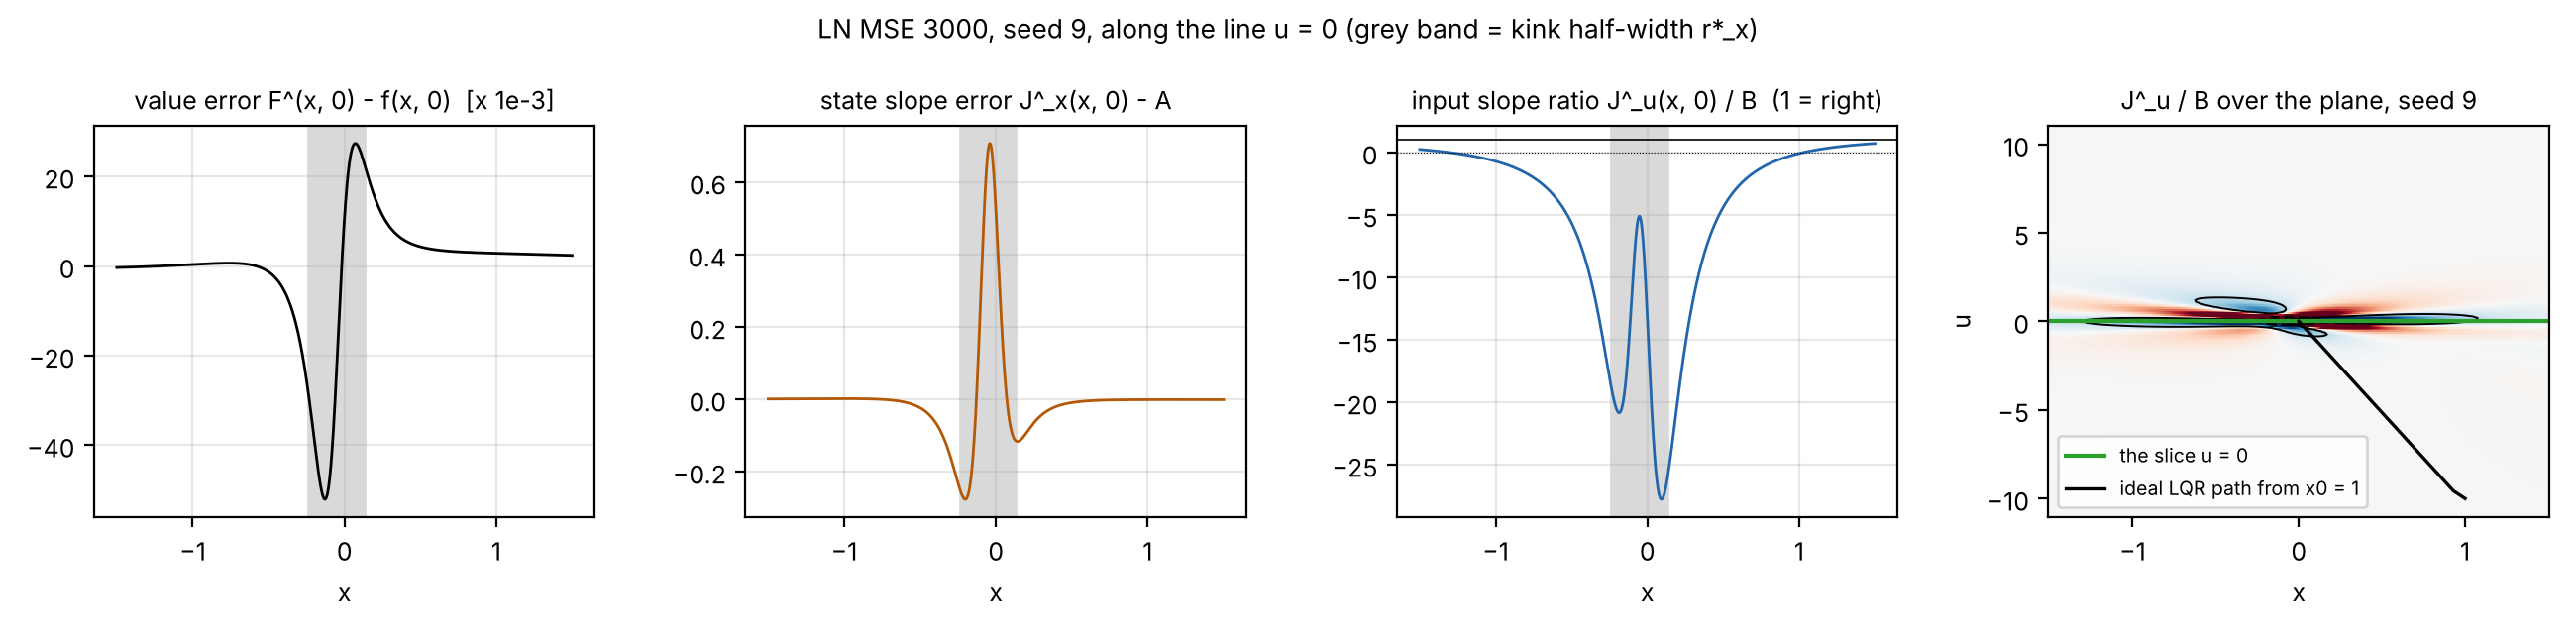
\includegraphics[width=\textwidth]{f03_fixed_u_slice.png}
\caption{Seed 9 of LN MSE 3000 along the line $u=0$, $|x|\le1.5$ (3001 points). Grey band: $|x-x^\star|\le r^*_x$. Panel 1: value error $\hat F-f$ in units of $10^{-3}$; it is a few $10^{-3}$ away from the kink and reaches about $0.05$ inside it. Panel 2: $\hat J_x-A$, a notch of $+0.7/-0.3$ confined to about two half-widths. Panel 3: $\hat J_u/B$; it is negative (wrong sign) along this whole line out to $|x|\approx1$, with minima of $-21$ and $-28$. Panel 4: the input-slope map over the plane with the slice (green) and the ideal LQR path from $x_0=1$ to $r=0$ (black), which crosses the plane steeply, not along the slice.}
\label{fig:slice}
\end{figure}

What the slice shows. A sharp notch in $\hat J_x$ at the origin, about two half-widths wide. It proves that the kink exists.

Why it cannot explain control failures.
\begin{enumerate}
\item A controller does not move along a line of constant $u$. A linear feedback $u=\hat u-K(x-r)$ moves along a line of slope $-K\approx-10$ in the $(x,u)$ plane (panel 4). The slopes it meets are those on that line, which the slice does not show.
\item The slope that matters most for these controllers is $\hat J_u$ (Section~\ref{sec:s7}), which a $\hat J_x$ slice does not display. On this very line, $\hat J_u$ has the wrong sign out to $|x|\approx1$, five to seven half-widths from the centre, while $\hat J_x$ is already back to normal beyond $|x|\approx0.3$. The $\hat J_x$ notch underestimates how far the defect reaches.
\item The slice has no notion of distance or direction in the plane, so it cannot say which setpoints or paths are at risk.
\end{enumerate}
Hypothesis at the time: the kink width $r^*_x$ along $x$ predicts the control damage. Observation: the damage correlated with the peak $\hat J_u$ error (Spearman 0.66, $p=0.04$, DPC study) and, for LQR, with the setpoint's distance from the kink in the plane (slides 11 to 12), neither of which the slice displays. Conclusion: move to two-dimensional maps of both slopes with the controller's path drawn on them. Every figure from slide 5 on uses that view.


%=====================================================================
\section{Slides 5 to 7: the Jacobian maps in 2-D and 3-D, the kink ellipse and the petals}\label{sec:s3}

\subsection{Colour convention used in every map}
Input-slope maps show the ratio $\hat J_u/B$ on a diverging scale centred at 1: white = 1 = correct; red = larger than $B$ (overestimated magnitude, up to the saturation value 5 in the colour scale); light blue = between 0 and 1 (underestimated); dark blue = below 0. The sign of $\hat J_u$ is wrong exactly inside the solid black contour $\hat J_u=0$. Red and blue are magnitudes relative to the truth, not signs. Some of the story figures (Figures~\ref{fig:four}, \ref{fig:swap9}, \ref{fig:swap8}) have a colour-bar label ``blue = wrong sign''; read it as ``below 1, and wrong sign inside the black contour''. State-slope maps show $\hat J_x-A$ on a purple-orange scale centred at 0 and saturating at $\pm0.5$; compare its colours with the stability margin $A-1=0.03$.

\begin{figure}[H]
\centering
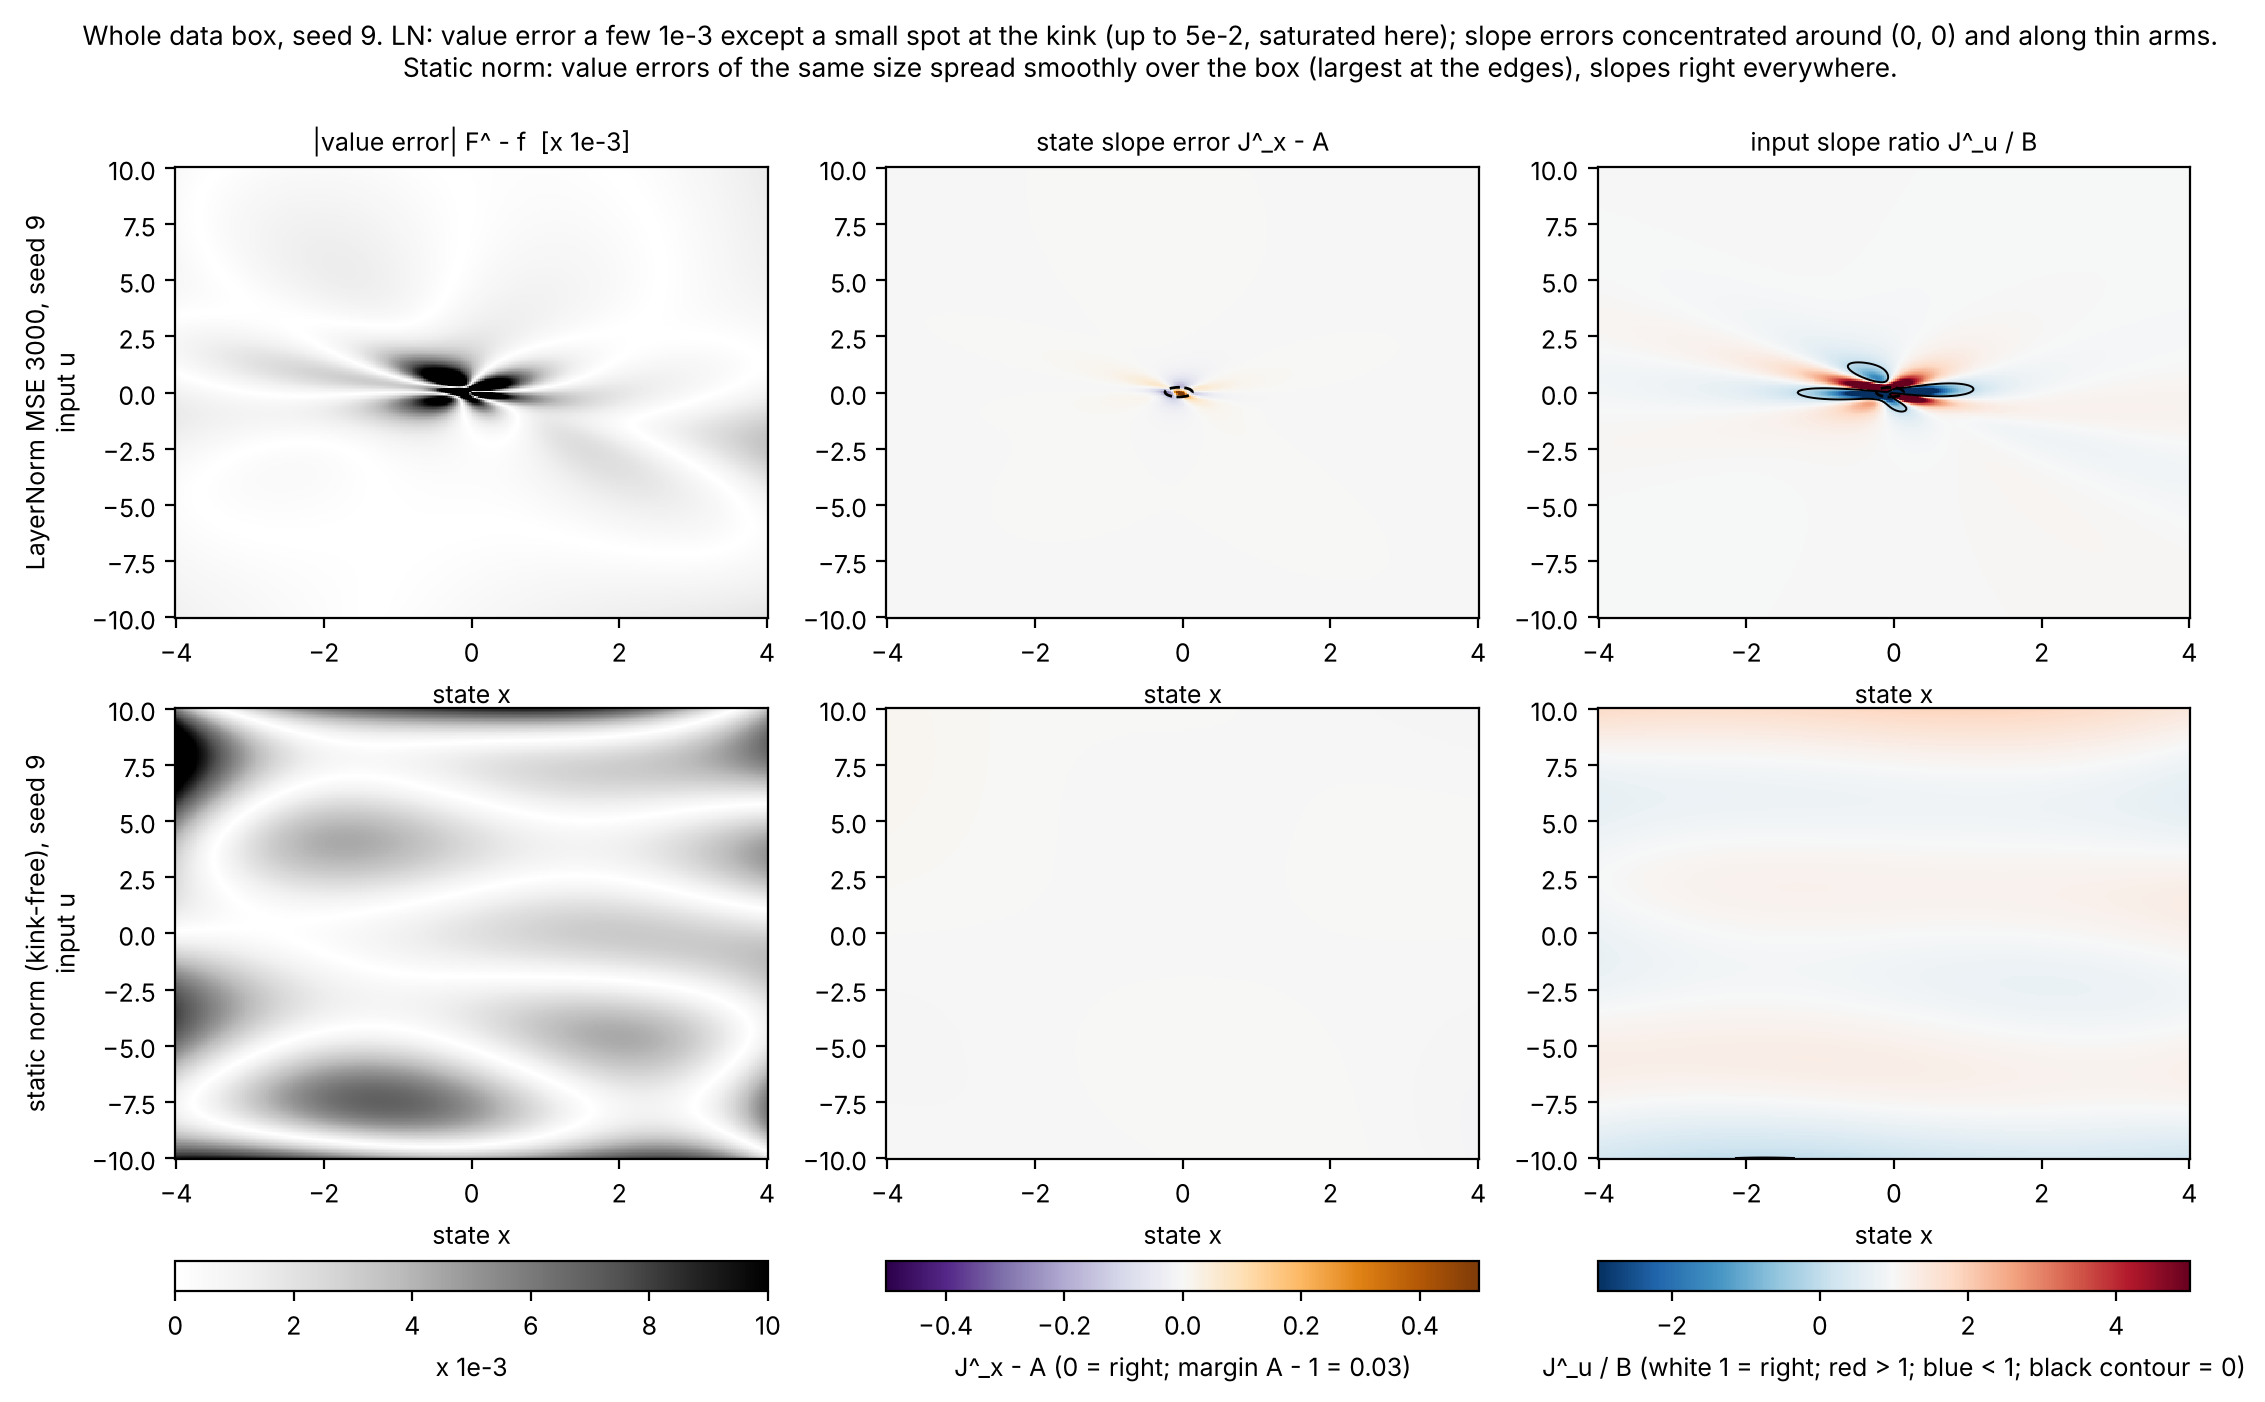
\includegraphics[width=\textwidth]{f04_maps_full_box.png}
\caption{Whole data box ($321\times321$ grid), seed 9. Top: LN MSE 3000. Bottom: static norm, same seed and data. Columns: absolute value error (saturated at $10^{-2}$), $\hat J_x-A$, $\hat J_u/B$. The LayerNorm surrogate's slope errors are concentrated around the origin and along thin arms; the static-norm surrogate has value errors of the same size spread smoothly over the box (largest near the edges) and input-slope errors below 100 percent everywhere (median over seeds of the maximum: 46 percent), with no wrong-sign region in the interior (for this seed a sliver at the box edge $u=-10$).}
\label{fig:fullbox}
\end{figure}

\begin{figure}[H]
\centering
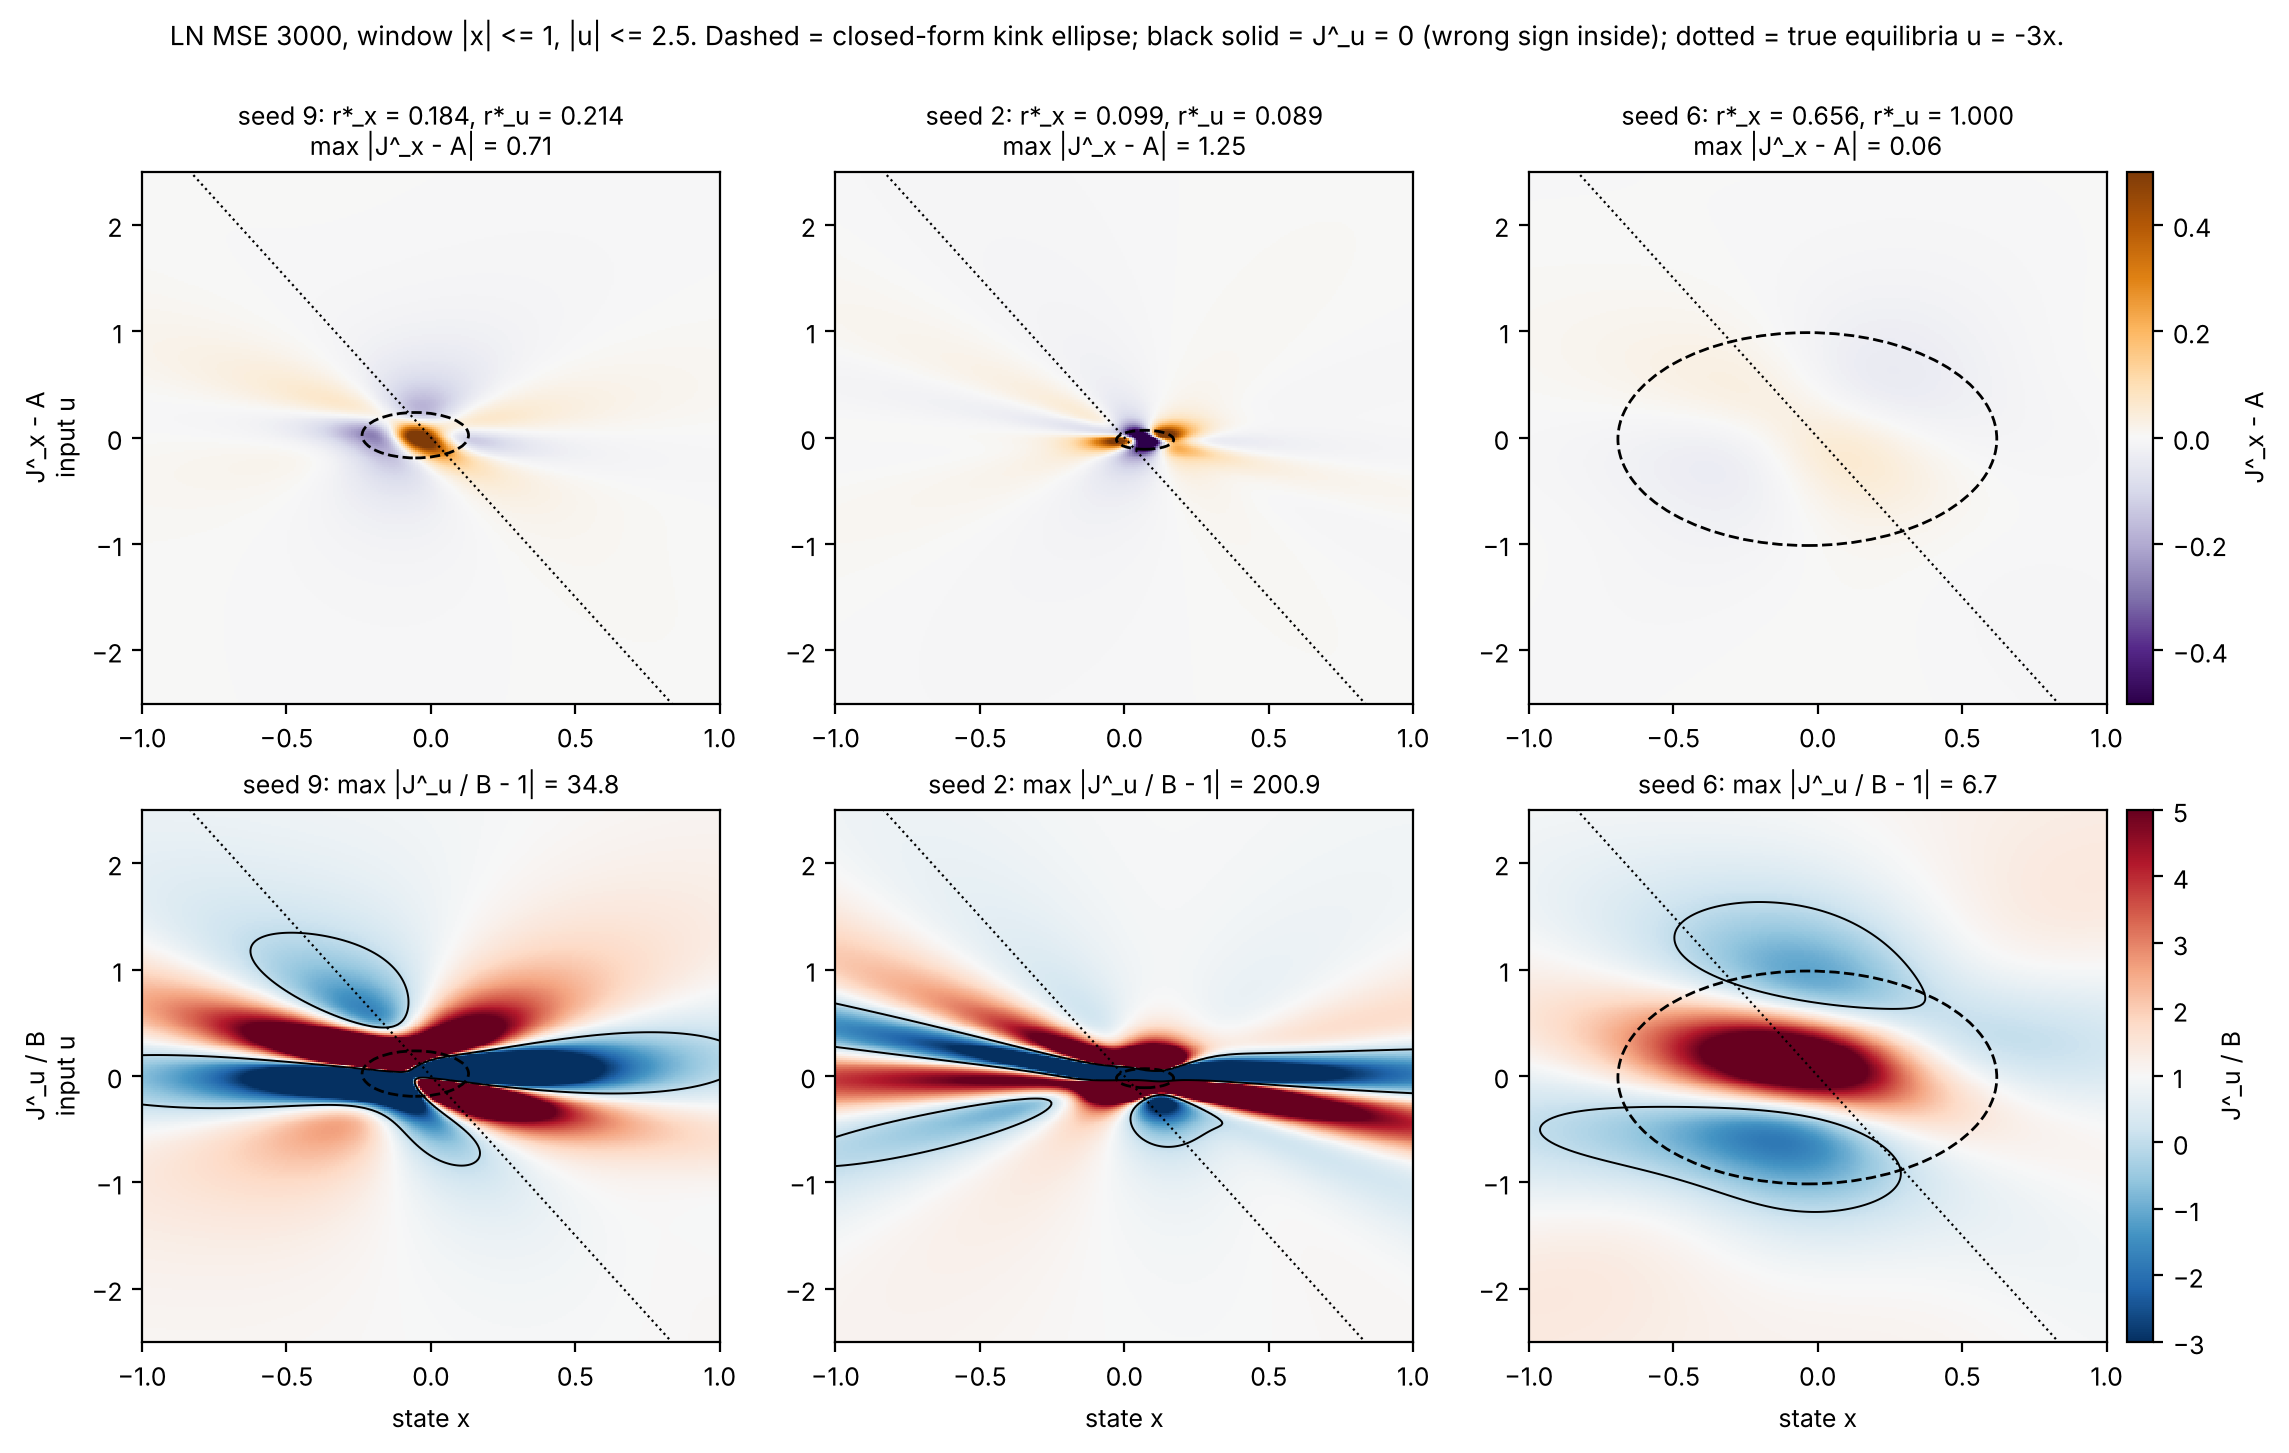
\includegraphics[width=\textwidth]{f05_maps_zoom.png}
\caption{Zoom $|x|\le1$, $|u|\le2.5$ ($281\times281$ grid) for three LN MSE 3000 seeds: 9 and 2 (narrow kinks) and 6 (the widest). Top: $\hat J_x-A$. Bottom: $\hat J_u/B$. Dashed: closed-form ellipse. Solid black: $\hat J_u=0$. Dotted: true equilibria $u=-3x$, i.e. where setpoints lie. The narrow kinks have the tallest errors (seed 2: $\hat J_u/B$ up to $-200$, $\hat J_x-A$ up to $1.25$) and arms of wrong sign that extend several half-widths along $u\approx0$; the wide kink of seed 6 has milder errors ($6.7$ and $0.06$) spread over a larger area. In every case the equilibrium line passes through the kink.}
\label{fig:zoom}
\end{figure}

\begin{figure}[H]
\centering
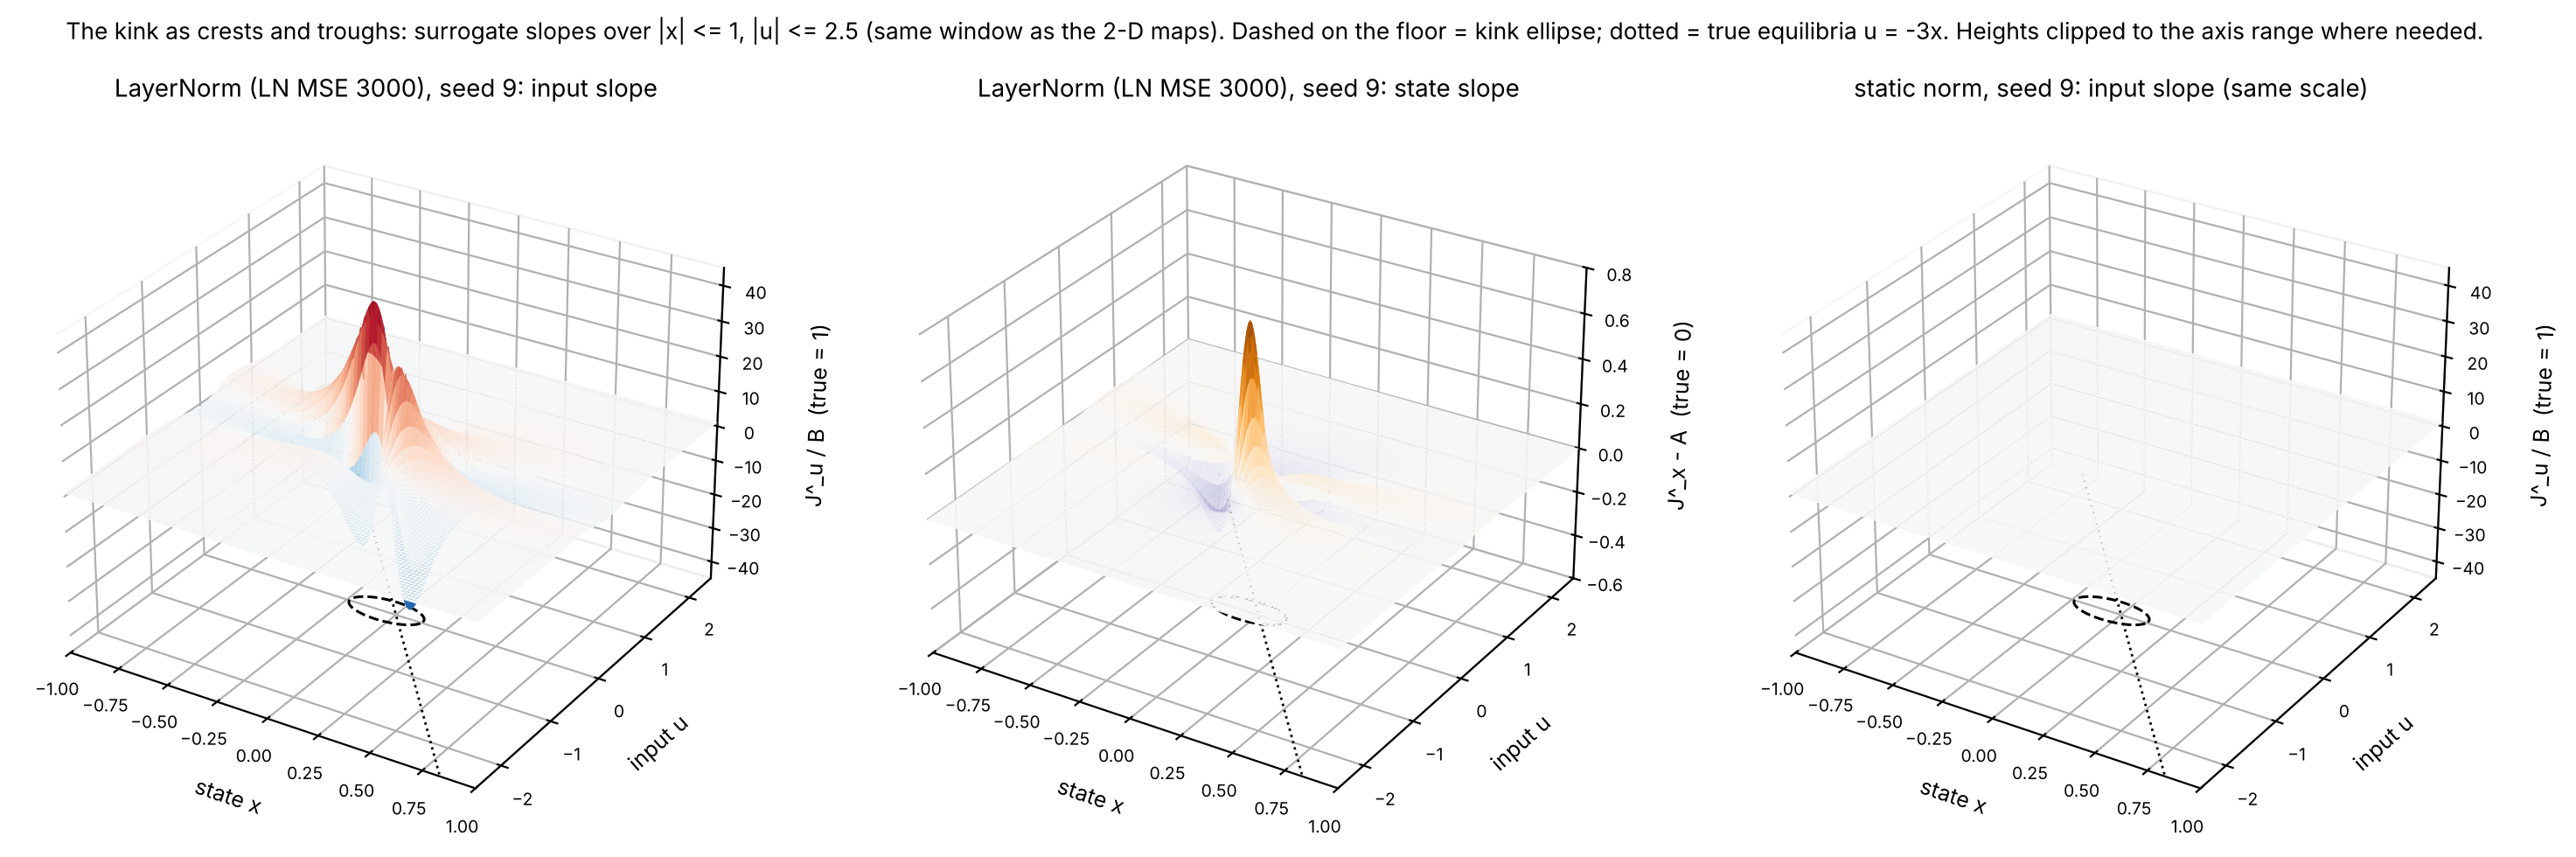
\includegraphics[width=\textwidth]{f16_slopes_3d.png}
\caption{Slide 6: the maps of Figure~\ref{fig:zoom} for seed 9 drawn as surfaces over the same window ($|x|\le1$, $|u|\le2.5$, $201\times201$ grid). Left: LN MSE 3000, $\hat J_u/B$ (true value 1). Middle: LN MSE 3000, $\hat J_x-A$ (true value 0). Right: static norm on the same seed and data, $\hat J_u/B$ on the same vertical scale as the left panel. Dashed ellipse on the floor: the closed-form kink ellipse; dotted: the true equilibria $u=-3x$. The LayerNorm input slope rises to $+41\,B$ on one side of the kink centre and falls to $-43\,B$ on the other, with lower ridges running out along the petals. The state slope has one sharp crest of $+0.71$ and a trough of $-0.28$. The static-norm input slope stays between $0.77\,B$ and $1.19\,B$ and looks flat at this scale.}
\label{fig:surf3d}
\end{figure}

How to read the surfaces (slide 6). The height is the slope itself. The true plant would be a flat sheet at height 1 in the left and right panels and at 0 in the middle panel. The two-dimensional maps clip their colour scales ($\hat J_u/B$ at $-3$ and $5$, $\hat J_x-A$ at $\pm0.5$), so they show where the slope is wrong but not by how much; the surfaces show the size. On seed 9 the input slope is a crest more than forty times the true value next to a trough of the opposite sign, both inside or right next to the kink ellipse, and the static-norm surface on the same data is a flat sheet. The same figure for the other seeds is produced by make\_fig3d.py with the seed as argument; the narrow seeds look similar with taller peaks (seed 2 reaches about $-200\,B$), the wide seeds have broader, lower relief.

Which crests and troughs belong to the kink. The surfaces also show smaller crests and troughs away from the centre, and not every bump is the kink. The kink is defined from the weights, not from the maps: it is the ellipse where LayerNorm's denominator is within a factor $\sqrt2$ of its minimum (Section~\ref{sec:kink}), and its centre and half-widths are known before any slope is computed. Outside it two different things appear.
\begin{itemize}
\item Petals, which are part of the kink. Away from the centre the normalised features depend almost only on the direction from $z^\star$, so the slope error is the angular change of the output divided by the distance, $\Phi'(\theta)/\rho$. The result is lobes that radiate from the kink centre, alternate in sign around it, and decay algebraically (Section~\ref{sec:kink}). They are the kink's long tails.
\item Ordinary fitting error, which is not. Every network has small, smooth slope wiggles. The kink-free surrogates have them too, but they are bounded (median over seeds of the largest $|\hat J_u/B-1|$: 0.46 for static norm, 0.77 for no norm), and they do not radiate from one point or follow a distance law.
\end{itemize}
Four checks separate the two:
\begin{center}
\footnotesize
\begin{tabular}{>{\raggedright\arraybackslash}p{3.2cm}>{\raggedright\arraybackslash}p{5.6cm}>{\raggedright\arraybackslash}p{5.2cm}}
\toprule
Check & Kink or petal & Other crests and troughs \\
\midrule
Location & centred on $z^\star$, predicted from $E$ and $b$ & anywhere, often near the box edges \\
Shape & lobes radiating from the centre, sign alternating & irregular, no radial pattern \\
Distance & amplitude falls off about as $1/d$ & no systematic decay \\
Same seed with static norm & absent & present at a similar size \\
\bottomrule
\end{tabular}
\end{center}
The last check is the cleanest: on the same seed and data, anything that survives replacing LayerNorm by static norm is a generic fitting artefact, and anything that disappears is LayerNorm's (compare the left and right panels of Figure~\ref{fig:surf3d}, or the two rows of Figure~\ref{fig:fullbox}). Size separates them too: kink peaks are 6.7 to 201 times $B$, while generic wiggles stay below about $1.2\,B$.

\begin{figure}[H]
\centering
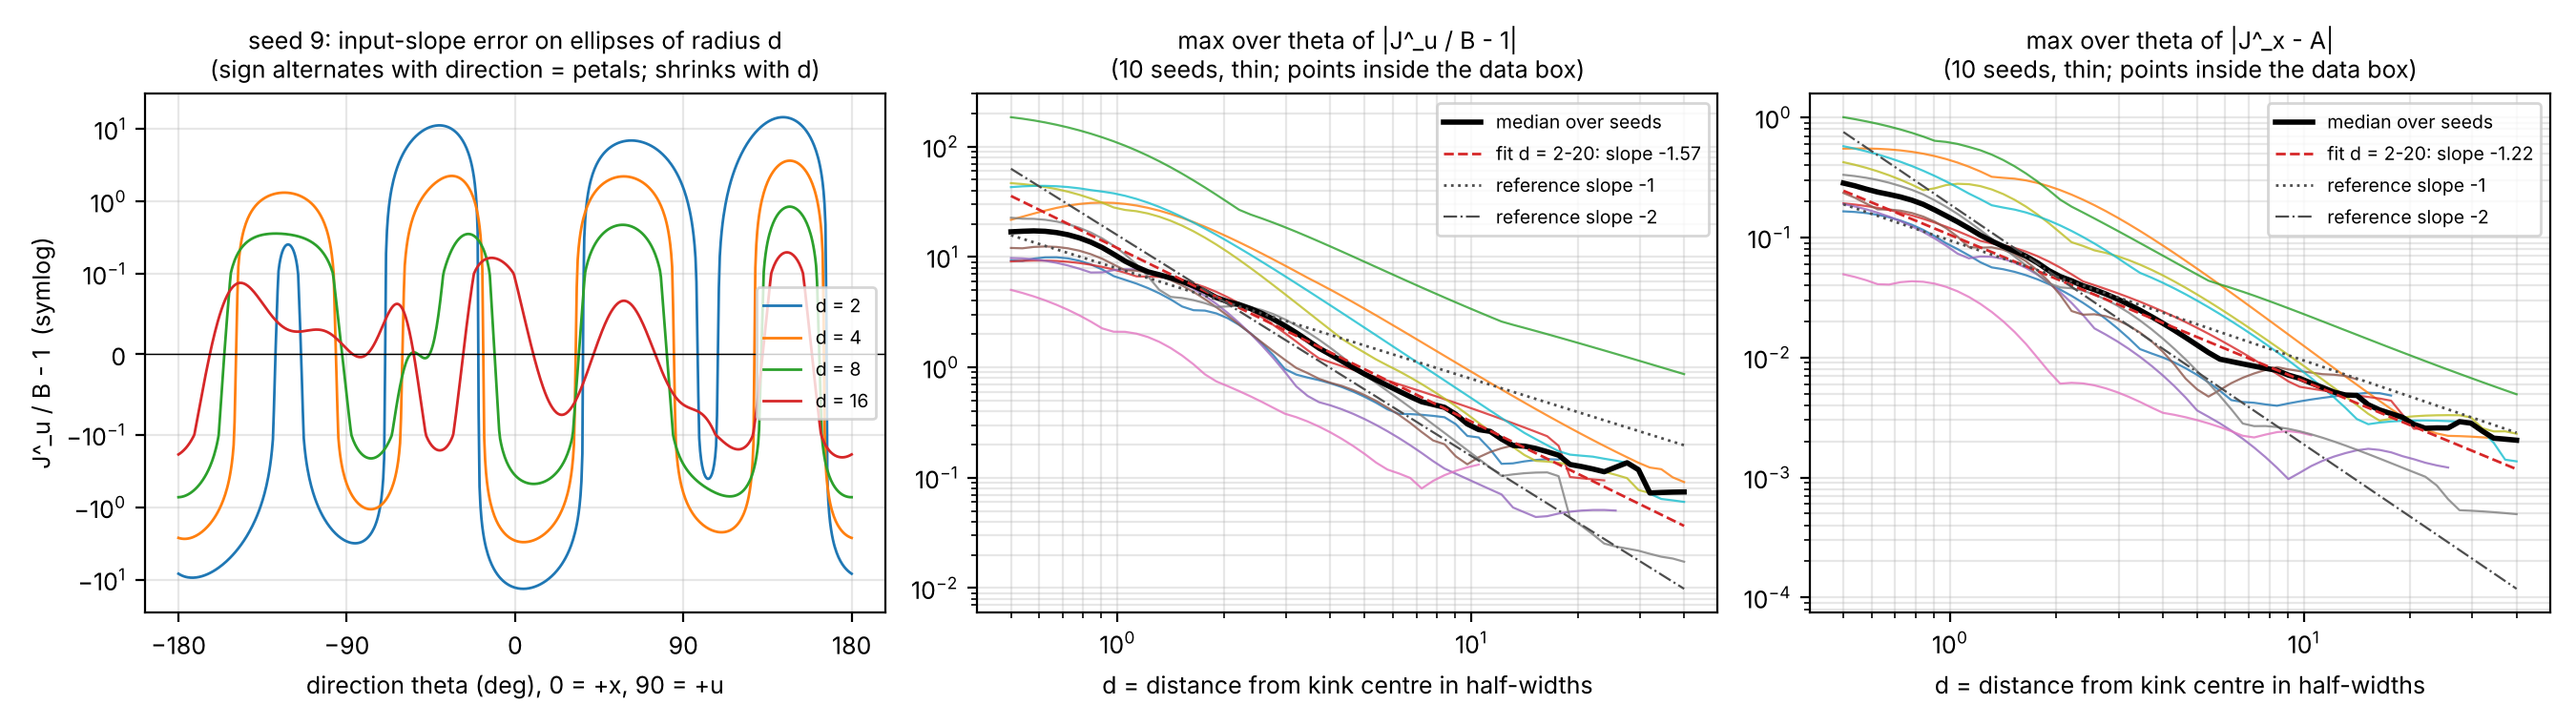
\includegraphics[width=\textwidth]{f06_petals_decay.png}
\caption{Petals and decay, LN MSE 3000. Left: $\hat J_u/B-1$ for seed 9 on ellipses of normalised radius $d=2,4,8,16$ around the kink centre ($x=x^\star+d\,r^*_x\cos\theta$, $u=u^\star+d\,r^*_u\sin\theta$), symlog scale. The sign alternates several times as the direction goes round (four positive and four negative lobes at $d=4$), and the amplitude shrinks with $d$. Middle and right: the largest error on each ellipse (points inside the data box only) against $d$, for all ten seeds (thin) and their median (thick), with reference slopes $-1$ and $-2$. Fit of the median over $d=2$ to $20$: slope $-1.57$ for $\hat J_u$ and $-1.22$ for $\hat J_x$. At $d\approx2$ the median input-slope error is still about 3 (300 percent); it falls below 10 percent only beyond $d\approx20$.}
\label{fig:petals}
\end{figure}

\subsection{Hypothesis, observation, conclusion}
Hypothesis (from Section~\ref{sec:kink}): LayerNorm's division by a data-dependent scale creates an ellipse of extreme slope error whose position and size follow from the first-layer weights alone, surrounded by lobes of alternating sign that decay algebraically.

Observations.
\begin{itemize}
\item On all ten seeds the ellipse computed from $E$ and $b$ sits on the measured hot spot (Figures~\ref{fig:fullbox} and \ref{fig:zoom}; centres within 0.1 of the origin, half-widths 0.10 to 0.66 in $x$ and 0.09 to 1.0 in $u$).
\item Both slopes are affected; $\hat J_u$ relative to $B$ far more (maxima 6.7 to 200.9 times $B$, median 18.7) than $\hat J_x$ relative to $A$ (0.06 to 1.25), but $\hat J_x$ errors are large compared with the margin 0.03.
\item Narrow kinks are taller (seed 2: $D=0.13$, peak 201; seed 6: $D=0.90$, peak 6.7), as the $1/D$ centre gain predicts.
\item Outside the ellipse the error alternates in sign with direction (petals) and decays algebraically: about $1/d$ along the equilibrium line (Figure~\ref{fig:law}), faster than $1/d$ but slower than $1/d^2$ for the largest error on a circle at $d=2$ to $20$ (Figure~\ref{fig:petals}). The wrong-sign arms reach 2 to 7 half-widths from the centre on 8 of 10 seeds (10 and 33 on the two narrowest, seeds 1 and 2); 56 to 99 percent of the wrong-sign area lies outside the kink ellipse. Along the setpoint line $u=-3x$ wrong-sign setpoint gains stop at about $d=4$, because the arms run mostly along $u\approx0$.
\item The kink-free static-norm surrogate has comparable value errors and no such structure.
\end{itemize}
Conclusion. The defect is structural (it comes from the normalisation, not from a lack of data or training), located (closed form from the weights), and long-ranged (algebraic tails). A controller does not need to enter the ellipse to be affected: setpoints two to four half-widths away still see input-slope errors of order one.

Why it matters. This is the mechanism half of the story. Everything after this slide asks how much of this geometry reaches a controller, and through which slope.

%=====================================================================
\section{Slide 8: fixed LQR, three numbers read once at the setpoint}\label{sec:s4}

\begin{figure}[H]
\centering
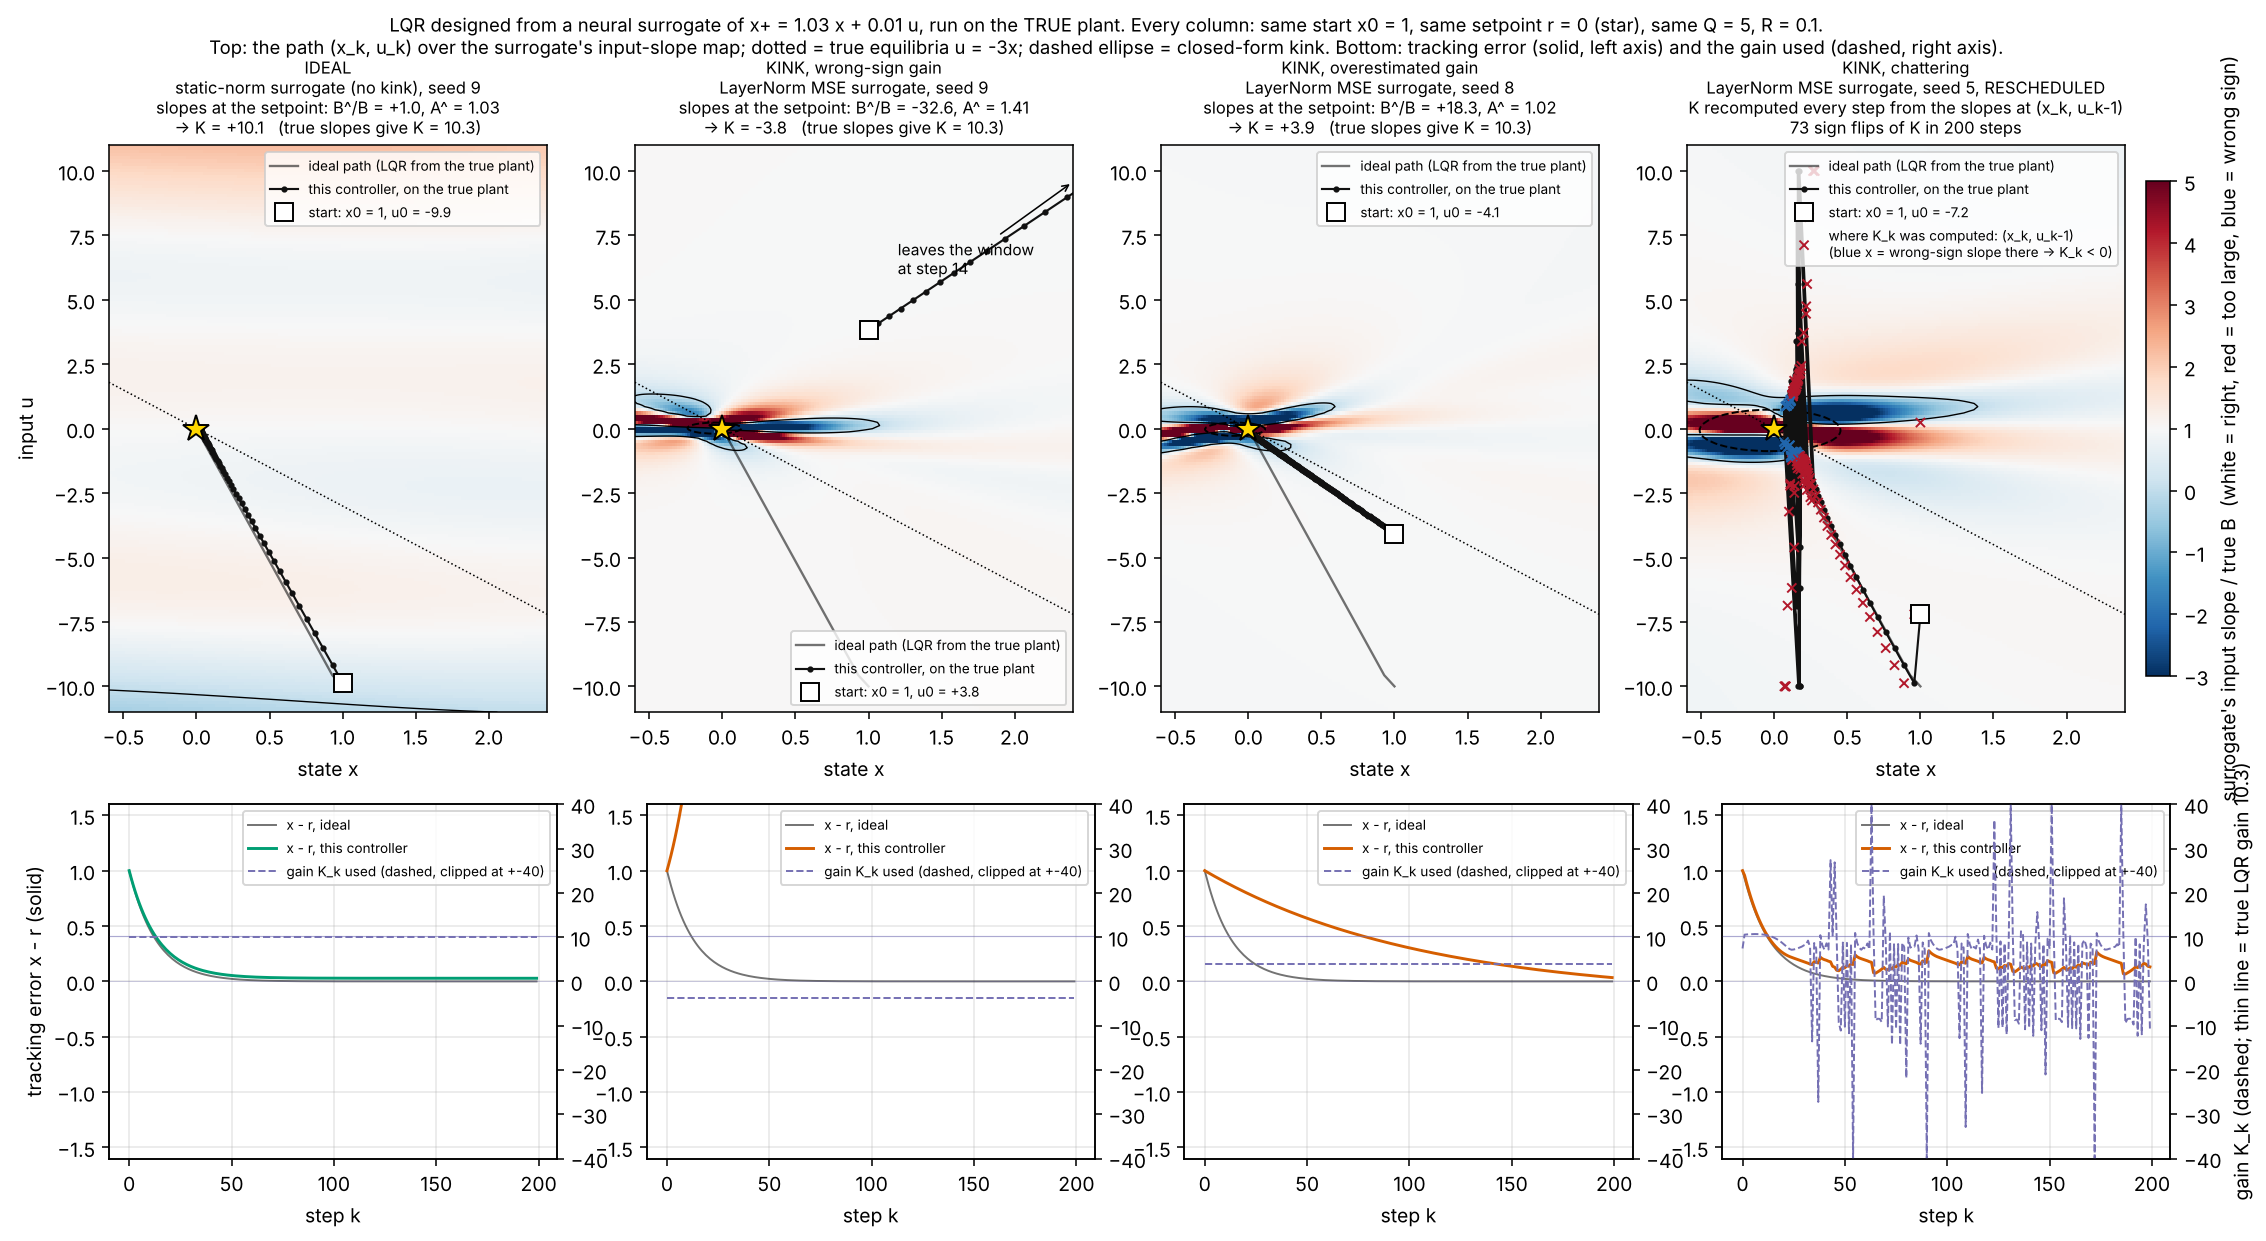
\includegraphics[width=\textwidth]{f07_lqr_four_cases.png}
\caption{Four LQR cases, all from $x_0=1$ to $r=0$ on the true plant, $Q=5$, $R=0.1$. Top row: the path $(x_k,u_k)$ (black dots) over the surrogate's input-slope map, the ideal path from the true-plant LQR (grey), start (square), setpoint (star), true equilibria (dotted), kink ellipse (dashed), $\hat J_u=0$ (solid black). Bottom row: tracking error $x_k-r$ (solid, left axis) and the gain $K_k$ used (dashed, right axis, clipped at $\pm40$; thin line = 10.29). Columns 1 to 3 are fixed LQR (slide 8); column 4 is the rescheduled LQR (slide 9). Surrogates: column 1 static norm, seed 9; columns 2 to 4 LN MSE 3000, seeds 9, 8 and 5; all trained with the MSE loss only for 3000 steps (Table~\ref{tab:fourcases}).}
\label{fig:four}
\end{figure}

\begin{figure}[H]
\centering
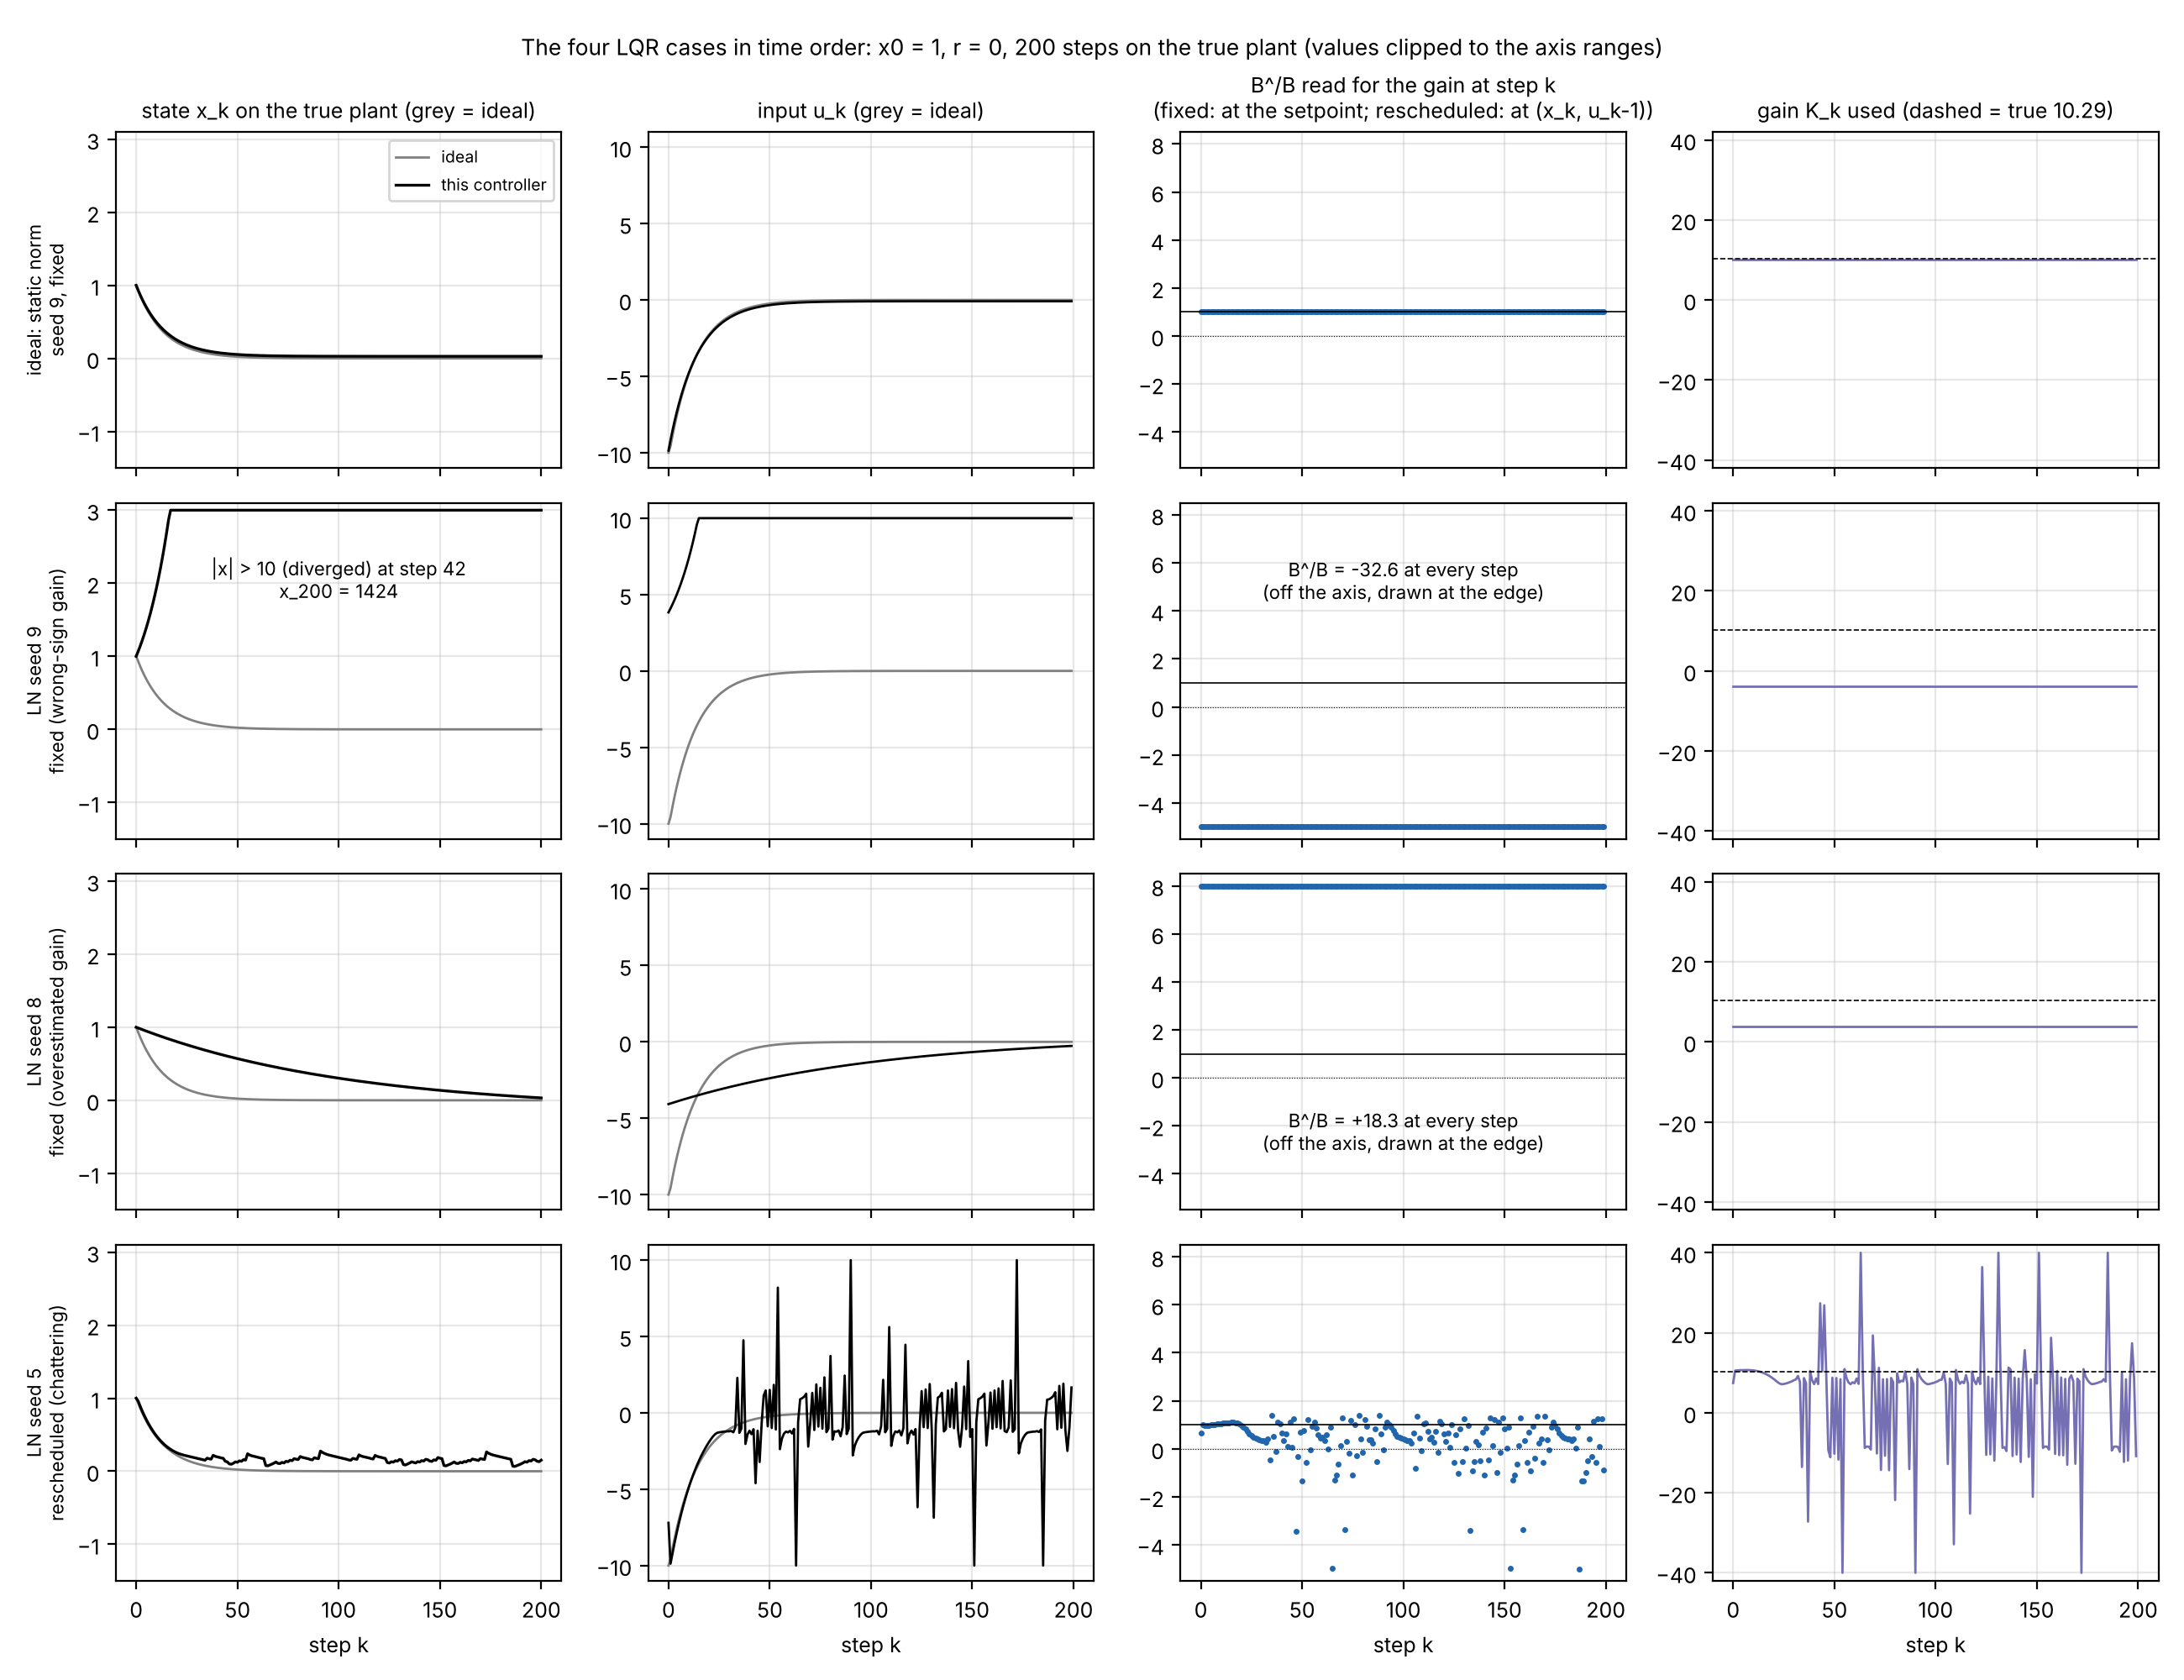
\includegraphics[width=\textwidth]{f08_lqr_timeline.png}
\caption{The same four cases in time order. Columns: state, input, the input slope ratio $\hat B/B$ that the gain at step $k$ was computed from, and the gain $K_k$. For the fixed LQR the slope and the gain are constant; values outside the axis ranges are drawn at the edge and their true values are written on the panel.}
\label{fig:timeline}
\end{figure}

\subsection{Which surrogate is in each column}
All four surrogates were trained with the value (MSE) loss only, for 3000 steps, on their seed's data; none has a slope loss. All four runs start at $x_0=1$ with setpoint $r=0$ on the true plant, with $Q=5$, $R=0.1$.
\begin{table}[H]
\centering
\footnotesize
\setlength{\tabcolsep}{4pt}
\begin{tabular}{lll>{\raggedright\arraybackslash}p{6.3cm}}
\toprule
Column & Surrogate & Controller & What it shows \\
\midrule
1 & static norm, MSE 3000, seed 9 & fixed LQR & ideal case: no kink, $K=10.06$, follows the oracle \\
2 & LN MSE 3000, seed 9 & fixed LQR & wrong-sign gain ($\hat B/B=-32.6$, $K=-3.79$): diverges \\
3 & LN MSE 3000, seed 8 & fixed LQR & overestimated slope ($\hat B/B=+18.3$, $K=3.94$): slow \\
4 & LN MSE 3000, seed 5 & rescheduled LQR & chattering across wrong-sign bands (Section~\ref{sec:s5}) \\
\bottomrule
\end{tabular}
\caption{The four cases of Figure~\ref{fig:four}.}
\label{tab:fourcases}
\end{table}
Column 1 uses the same seed as column 2 on purpose: the same training data, the same initialisation and the same MSE training, with static norm in place of LayerNorm. The difference between columns 1 and 2 is therefore the normalisation alone.

\subsection{How to read the three fixed-LQR columns}
The fixed-LQR path in the $(x,u)$ plane is a straight line by construction: $u=\hat u-K(x-r)$ is affine in $x$, a line of slope $-K$ through $(r,\hat u)$, until it hits the input limit. The slope of that line is the gain. Q and R only set the ideal slope.

Column 1, ideal (static norm, seed 9). At the setpoint the surrogate gives $\hat B/B=1.02$, $\hat A=1.029$, $\hat u=0.20$, so $K=10.06$. The first input is $u_0=-9.86$ (close to the limit, as in the oracle, because $B$ is small) and the state reaches the setpoint in about 50 steps along the ideal line.

Column 2, wrong-sign gain (LN MSE 3000, seed 9). The setpoint lies inside the black contour: $\hat B/B=-32.6$ and $\hat A=1.41$. The Riccati gain takes the sign of $\hat A\hat B$, so $K=-3.79$. The controller pushes the wrong way: $u_0=+3.83$, the true closed loop is $x_{k+1}=(1.03+0.0379)x_k+0.01\hat u$, i.e. a pole of 1.068. The input reaches the limit $+10$ at step 15, after which $x_{k+1}=1.03x_k+0.1$ grows without bound; $|x|>10$ at step 42. Catastrophic.

Column 3, overestimated gain (LN MSE 3000, seed 8). The setpoint lies on a red petal: $\hat B/B=+18.3$, $\hat A=1.022$, so $K=3.94$ instead of 10.29. The true pole is $1.03-0.0394=0.991$: stable but slow, with a time constant of about 106 steps instead of 13. The state creeps towards the setpoint ($x_{200}=0.033$) and the cost is far above the oracle. Failed, not diverged.

The scalar intuition behind all three: $K$ has the sign of $\hat B$ and falls as $\hat B$ grows, but much more slowly than $1/\hat B$ ($\hat B=18.3B$ gives $K=3.99$ with the true $A$, a factor 2.6, not 18). A wrong-sign $\hat B$ gives $K<0$ and divergence. An overestimated $\hat B$ gives a small $K$; the loop on the true plant has pole $1.03-0.01K$, which is harmless until $K$ drops below about 3 (pole $\ge1$), i.e. $\hat B/B$ above about 30 (example: seed 1 at $r=0.1$, $\hat B/B=29$, $K=3.0$, gap 560 percent). An underestimated $\hat B$ gives a large $K$, aggressive inputs that saturate, and a higher cost.

\subsection{Hypothesis, observation, conclusion}
Hypothesis H1: a fixed LQR is damaged exactly when its design point $(r,\hat u(r))$ lies on the kink or on a petal, and the type of damage follows from the local $\hat J_u/B$ there.

Observations (880 runs per family).
\begin{itemize}
\item All 72 runs (over the four LayerNorm families) whose setpoint gain had the wrong sign diverged.
\item LN MSE 3000: 26.5 percent of runs failed, 10.8 percent catastrophically. Static norm: 0.6 and 0 percent. No norm: 2.6 and 0. LN MSE 12000: 6.5 and 1.1. LN slope from step 0: 5.8 and 1.4. LN two-stage: 5.7 and 0.9.
\item Per seed (Table~\ref{tab:seeds}), the four narrowest kinks (seeds 1, 2, 8, 9) have catastrophic rates of 20 to 28 percent; the middle-width seeds 3, 4, 7 have none; the three widest (seeds 0, 5, 6) fall in between (1.1 to 9.1 percent), because their milder errors cover more setpoints. Width alone does not predict the catastrophic rate: every seed with a wrong-sign setpoint gain (0, 1, 2, 8, 9) has 9 to 28 percent catastrophic runs, every seed without one (3 to 7) has 0 to 3.4 percent.
\end{itemize}
Conclusion. For a fixed design the kink acts through one point. Reading the surrogate's input slope at the setpoint predicts the outcome. This is the simplest and most defensible demonstration that the kink reaches control: a textbook linearise-and-design procedure, applied to an accurate model exactly as a practitioner would, fails because of a derivative defect at a predictable location.

%=====================================================================
\section{Slides 9 to 10: rescheduled LQR, reading the slopes along the path}\label{sec:s5}

\begin{figure}[H]
\centering
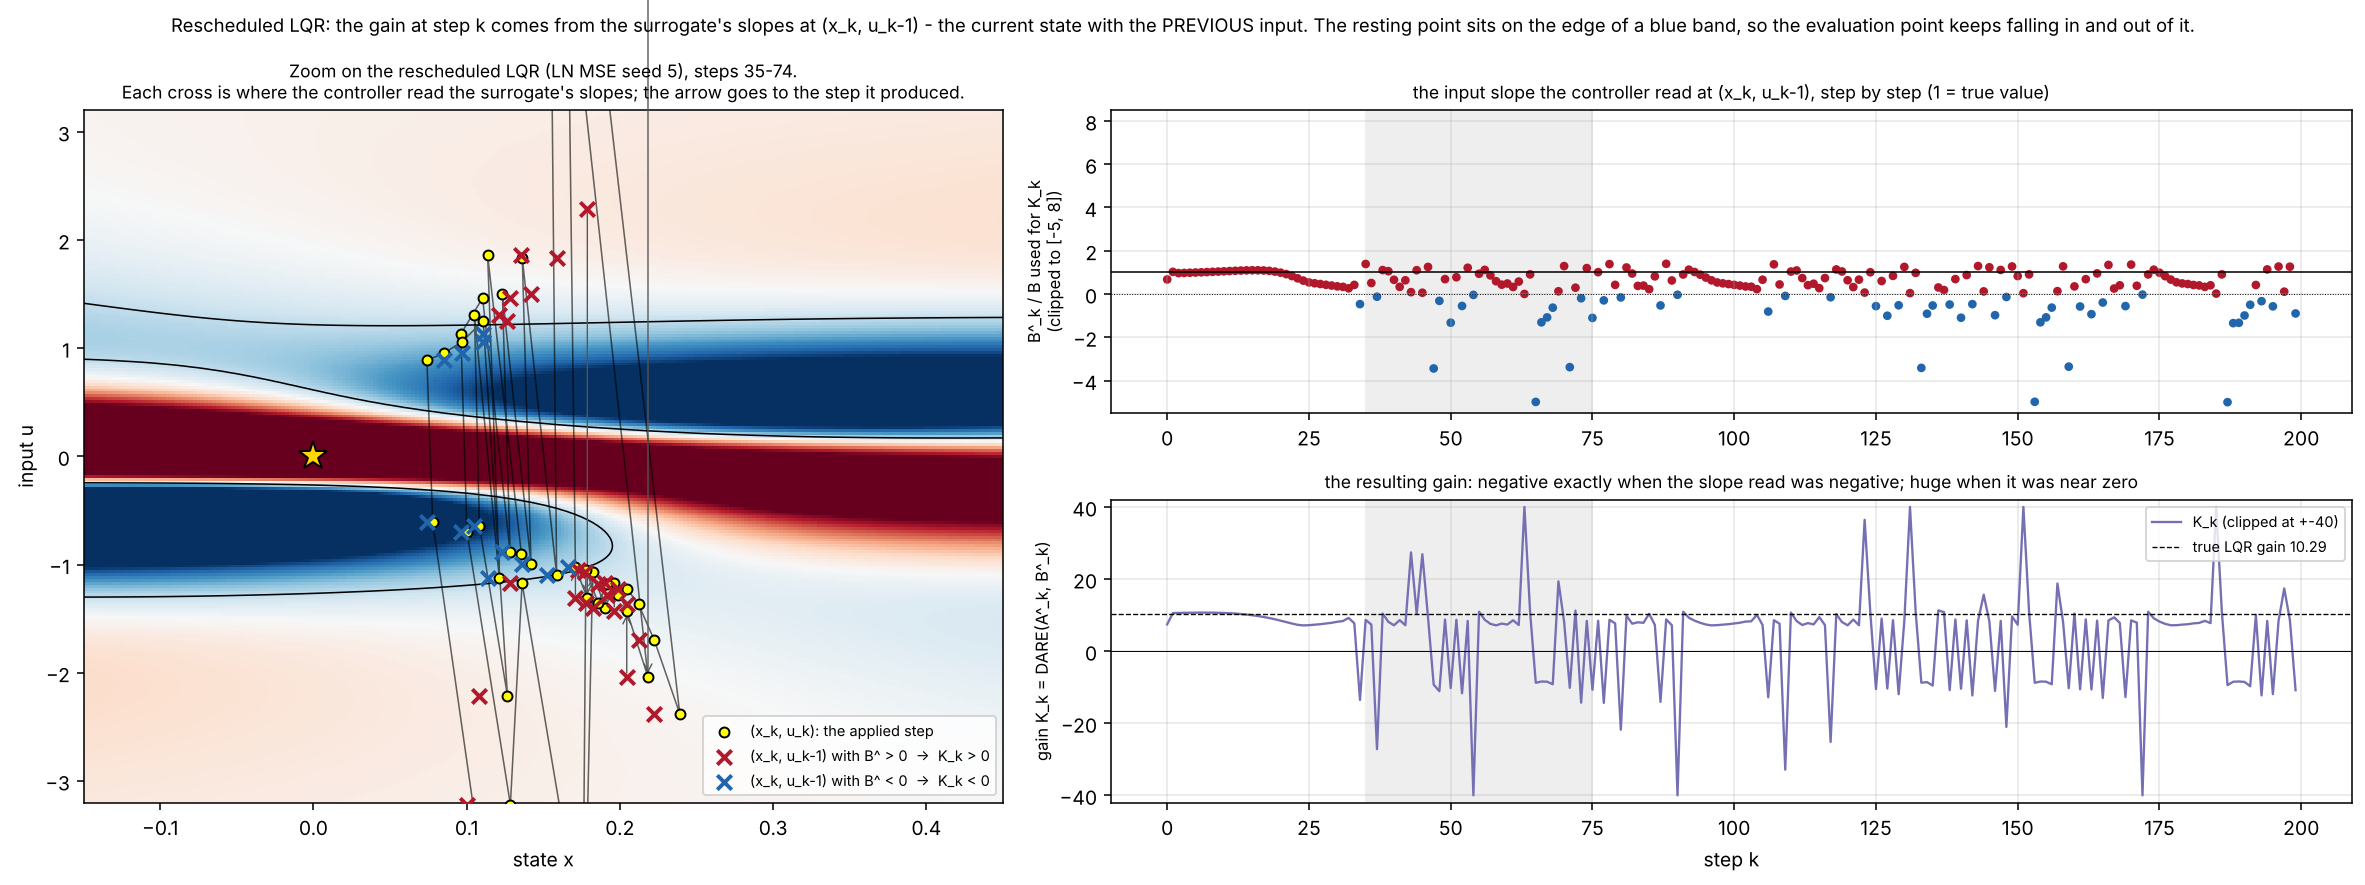
\includegraphics[width=\textwidth]{f09_rescheduled_zoom.png}
\caption{The rescheduled LQR of Figure~\ref{fig:four}, column 4 (LN MSE 3000, seed 5, $x_0=1$, $r=0$). Left: steps 35 to 74 near the resting point. Yellow dots are the applied points $(x_k,u_k)$; crosses are the points $(x_k,u_{k-1})$ where the slopes for $K_k$ were read, red if $\hat B>0$ there (so $K_k>0$) and blue if $\hat B<0$ (so $K_k<0$); thin lines join each evaluation point to the step it produced. Right: $\hat B_k/B$ read at each step (top) and the resulting gain $K_k$ (bottom, clipped at $\pm40$; dashed = 10.29); the shaded interval is the zoom on the left.}
\label{fig:resched}
\end{figure}

\subsection{How to read it}
The path is no longer a line, because each step uses a different gain. In Figure~\ref{fig:four} (column 4) the first steps follow the ideal path, then near the setpoint the evaluation points start to fall into the wrong-sign bands just below and above $u=0$ (blue crosses in Figure~\ref{fig:resched}). Whenever $\hat B_k<0$ the gain flips sign ($K_k<0$), $u_k$ jumps to the other side, the next evaluation point lands on a red or near-zero region where $K_k$ is large, and the input jumps back. The result is chattering: 73 sign flips of $K$ in 200 steps, inputs hitting $\pm10$, and a resting point about 0.15 away from the setpoint. Seed 5 is not one of the worst seeds for the fixed LQR (its setpoint gain gives $K=6.96$); it fails here because its path crosses the petals.

\begin{figure}[H]
\centering
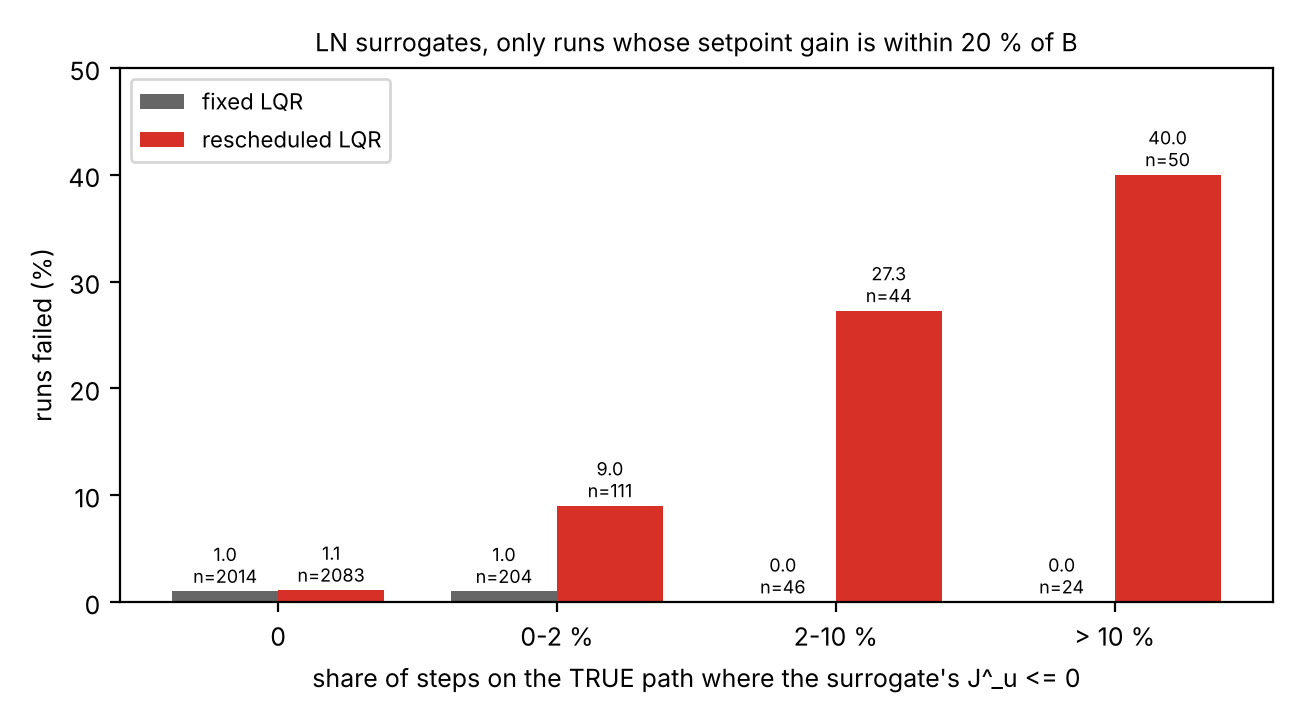
\includegraphics[width=0.7\textwidth]{f10_path_colour_test.png}
\caption{Path-colour test. LayerNorm surrogates only, and only runs whose setpoint gain is within 20 percent of $B$ (so the setpoint cannot be blamed). Runs are grouped by the share of the 200 steps of each run's own path on the true plant at which the surrogate's $\hat J_u\le0$ (Section~\ref{sec:s5}, ``How the path-colour test was done''). Bars: failure rate of the fixed LQR (grey) and the rescheduled LQR (red), with the number of runs in each group.}
\label{fig:pathcolour}
\end{figure}

\subsection{How the path-colour test was done}
The test runs no new simulations. It re-slices the runs of the LQR study (Section~\ref{sec:eval}) as follows.
\begin{enumerate}
\item Surrogates: the four LayerNorm families (LN MSE 3000, LN MSE 12000, LN slope from step 0, LN two-stage), ten seeds each, 40 surrogates in total. The two kink-free families are not part of this test.
\item Runs: for every surrogate, the 11 setpoints and 9 starts of Section~\ref{sec:grids} with $|x_0-r|\ge0.5$, i.e.\ 88 runs per seed and 3520 runs in total. Each run is simulated twice on the true plant for 200 steps, once with the fixed LQR and once with the rescheduled LQR built from that surrogate, and the visited points $(x_k,u_k)$, $k=0,\dots,199$, are stored. Every run is deterministic.
\item Failure: a run failed if its cost gap against the oracle LQR from the same $(r,x_0)$ exceeds 10 percent or it diverged (Section~\ref{sec:eval}).
\item Wrong-sign share of a run: the surrogate's input slope is evaluated by automatic differentiation at each of the 200 visited points, and
\begin{equation}
\text{wrong-sign share} = \frac{1}{200}\,\#\{k:\ \hat J_u(x_k,u_k)\le0\},
\end{equation}
the fraction of the run's steps that lie on the wrong-sign (dark blue) region of the input-slope map (function seen\_gain in phase\_core.py, then \texttt{wrong = (ju <= 0).mean(0)}).
\item Control filter: only runs whose setpoint slope is close to the truth are kept, $|\hat B(r)/B-1|\le0.2$ at $(r,\hat u(r))$. This removes every run in which the fixed LQR starts from a bad gain, so a failure in the remaining runs cannot be blamed on the setpoint. The filter depends only on the surrogate and the setpoint, so the same 2288 of the 3520 combinations (65 percent) are kept for both controllers.
\item Groups: each kept run is placed in one of four groups by its wrong-sign share:
\begin{center}
\begin{tabular}{lll}
\toprule
Group & Wrong-sign share & Wrong-sign steps out of 200 \\
\midrule
0 & exactly 0 & none \\
0 to 2 percent & above 0, at most 0.02 & 1 to 4 \\
2 to 10 percent & above 0.02, at most 0.10 & 5 to 20 \\
over 10 percent & above 0.10 & 21 or more \\
\bottomrule
\end{tabular}
\end{center}
For example, a run that touches the wrong-sign region at 12 of its 200 points has a share of 0.06 and falls in the 2 to 10 percent group. 88 to 91 percent of the kept runs (2014 of 2288 for the fixed LQR, 2083 for the rescheduled LQR) never touch a wrong-sign point, so the first group is a clean baseline. The edges 0.02 and 0.10 are judgement calls.
\item Rates: within each group, the percentage of runs that failed, counted separately for the two controllers. The group sizes $n$ differ between the controllers because each run is grouped by the path its own controller took. (The study is run by lqr\_study in phase\_core.py through run\_lqr\_study.py; the filter, grouping and figure are the ``F10 path-colour test'' block of make\_figs.py.)
\end{enumerate}

Check against reverse causation. Grouping by each controller's own path allows failure to feed back into the grouping: a rescheduled run that starts chattering near the kink spends more steps on the wrong-sign region because it is failing. To remove this, the same kept runs were also grouped by the wrong-sign share along the oracle's path from the same $(r,x_0)$, which neither controller influences. The result is unchanged (no oracle path has a share above 10 percent, so the last group is empty):
\begin{center}
\begin{tabular}{lccc}
\toprule
Grouped by the oracle's path & 0 & 0 to 2 percent & 2 to 10 percent \\
\midrule
fixed LQR, failed (\%) & 1.0 & 0.5 & 1.6 \\
rescheduled LQR, failed (\%) & 1.2 & 11.5 & 25.4 \\
$n$ (both controllers) & 2016 & 209 & 63 \\
\bottomrule
\end{tabular}
\end{center}

Limitations of the test. The share is measured at the applied points $(x_k,u_k)$, whereas the rescheduled LQR reads its slopes at $(x_k,u_{k-1})$; the two are close except during chattering. The upper groups are small (24 to 63 runs, from a few seeds), so the trend across groups is clear but the individual percentages are rough. The filter threshold and the group edges were chosen after the runs existed; other reasonable choices should be shown to give the same trend.

\subsection{Hypothesis, observation, conclusion}
Hypothesis H2: a controller that consults the slopes along its path is damaged by the petals that its path crosses, independently of the slope at the setpoint; a controller that reads the slopes only at the setpoint is not.

Observations.
\begin{itemize}
\item Path-colour test (Figure~\ref{fig:pathcolour}): as the wrong-sign share of the path grows through 0, 0 to 2, 2 to 10 and over 10 percent, the fixed LQR fails on 1.0, 1.0, 0 and 0 percent of runs ($n=2014$, 204, 46, 24) and the rescheduled LQR on 1.1, 9.0, 27.3 and 40.0 percent ($n=2083$, 111, 44, 50).
\item Over all runs, LN MSE 3000: the rescheduled LQR fails on 20.5 percent (3.4 percent catastrophic) against 26.5 (10.8) for the fixed LQR. Its failures form a wider band over setpoints (Figure~\ref{fig:setpoint}, right: 26 to 35 percent for $|r|\le0.25$, about 30 percent at $r=-0.5$, 9 to 12 percent at $|r|=0.5$ to 1, 2 percent at $|r|=2$).
\item Its catastrophic rate is lower than the fixed LQR's because re-reading the slopes lets it recover from a bad setpoint gain once the state moves off the setpoint; in exchange it is hurt wherever its path goes.
\item Kink-free and slope-trained surrogates: 0.8 to 5.7 percent failed. One exception that is not a kink effect: all 32 catastrophic rescheduled runs of the no-norm family come from one seed (8), from negative starts, settling about 1.5 below the setpoint with no wrong-sign slopes on the path. Re-linearising a smooth but imperfect model can create false resting points; this was not analysed further.
\end{itemize}
Conclusion. The same surrogate harms a fixed design through one point and a scheduled design through its whole path. Whether the colours along the path matter depends on whether the controller uses the slopes along the path. The long petals are what let path-dependent damage reach setpoints far from the ellipse.

Why it matters. It is the bridge to DPC. The rescheduled LQR is the simplest controller whose outcome depends on the slopes at many points; DPC depends on the slopes at every point of every training rollout.

%=====================================================================
\section{Slides 11 to 12: the setpoint law}\label{sec:s6}

\begin{figure}[H]
\centering
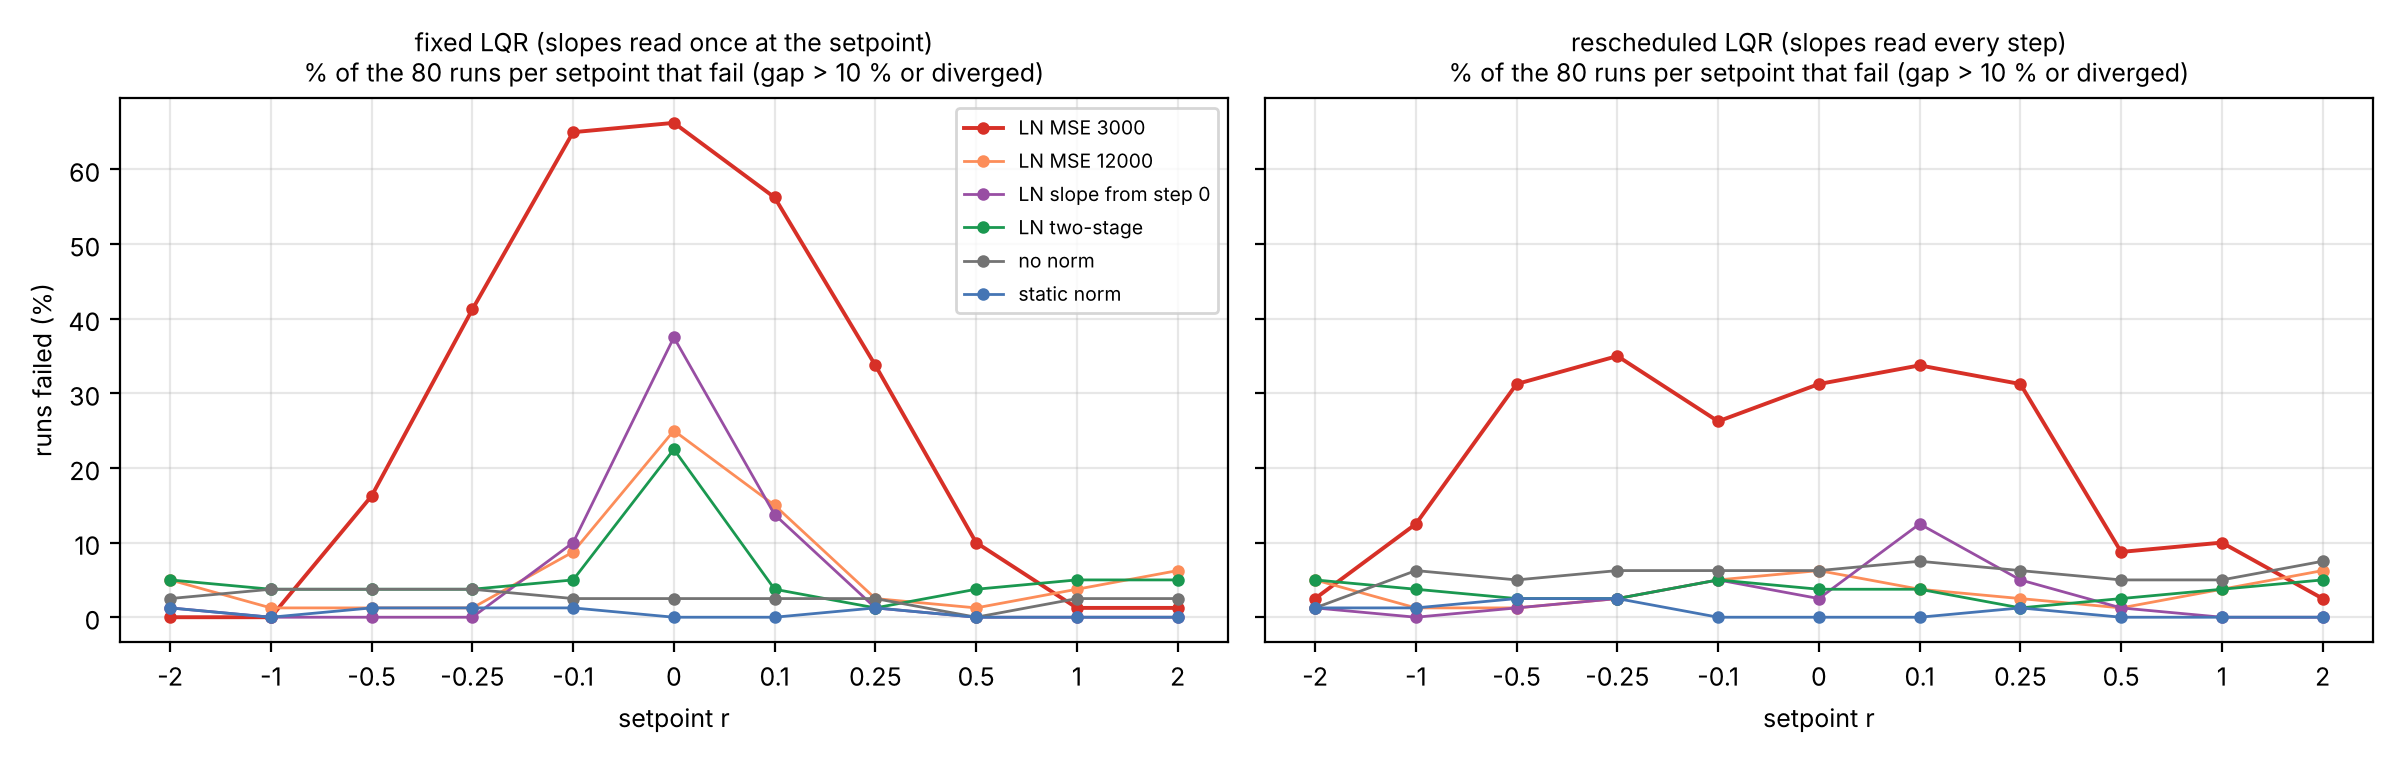
\includegraphics[width=\textwidth]{f11_failure_vs_setpoint.png}
\caption{Failure rate against setpoint for the six families: fixed LQR (left) and rescheduled LQR (right). Each point is the percentage of the 80 runs at that setpoint (10 seeds $\times$ 8 starts with $|x_0-r|\ge0.5$) that failed. The setpoint axis is categorical.}
\label{fig:setpoint}
\end{figure}

\begin{figure}[H]
\centering
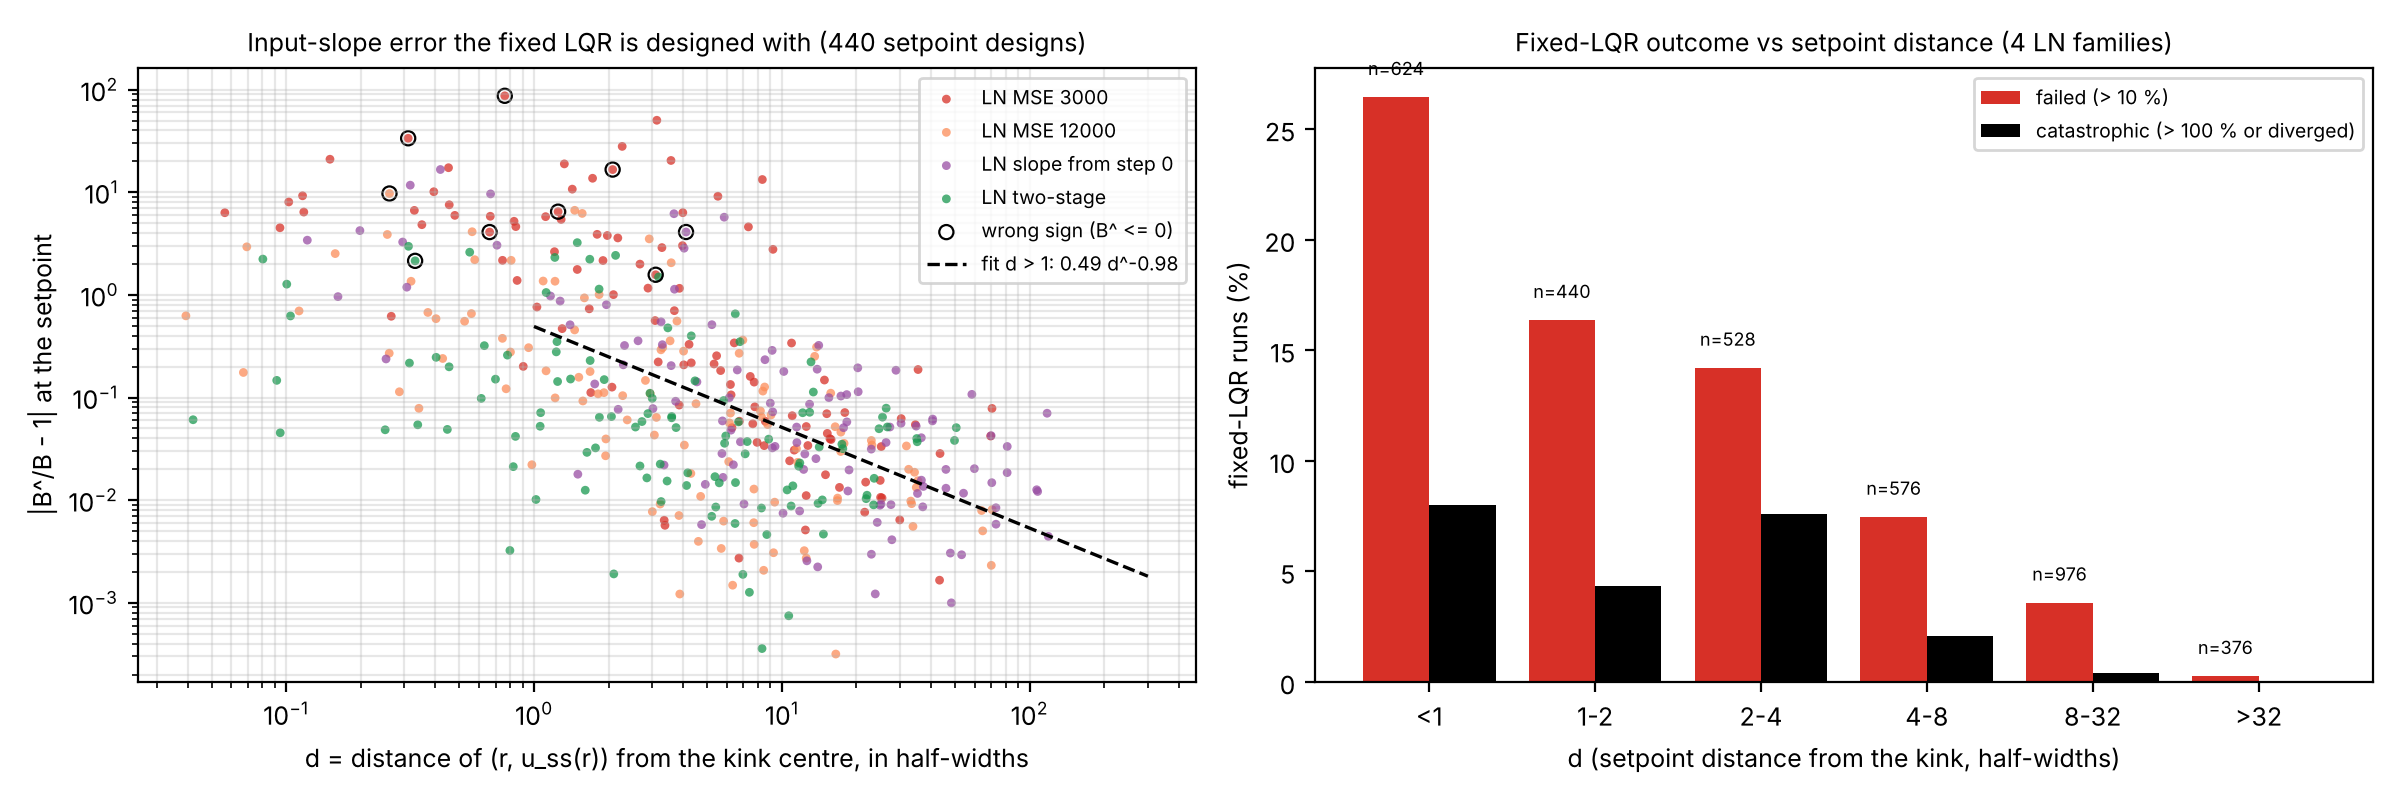
\includegraphics[width=\textwidth]{f12_setpoint_law.png}
\caption{Left: the input-slope error the fixed LQR is designed with, $|\hat B/B-1|$ at $(r,\hat u(r))$, against the setpoint distance $d$ from the kink centre in half-widths, for the four LayerNorm families (10 seeds $\times$ 11 setpoints each). Open circles mark wrong-sign setpoint gains. Dashed: least-squares fit in log-log coordinates over $d>1$. Right: fixed-LQR failure and catastrophic rates by distance bin (all runs of the four LayerNorm families with $|x_0-r|\ge0.5$; $n$ = runs per bin).}
\label{fig:law}
\end{figure}

\subsection{The law}
\begin{equation}
\Big|\frac{\hat B(r)}{B}-1\Big| \approx 0.49\,d^{-0.98}\qquad(d>1),\qquad d=\sqrt{\Big(\frac{r-x^\star}{r^*_x}\Big)^2+\Big(\frac{u_{ss}(r)-u^\star}{r^*_u}\Big)^2}.
\end{equation}
This is the petal tail of Section~\ref{sec:kink} measured at the operating points a fixed LQR would use. The fit is over 440 setpoint designs from four families, so the scatter is large (about one decade at a given $d$); the product $d\cdot|\hat B/B-1|$ has medians of 0.32 to 0.71 across distance bins. Median errors: 51 percent at $d=1$ to 2, 18 percent at 2 to 4, 5 percent at 4 to 8, 3 percent at 8 to 32. Wrong-sign setpoint gains occur out to $d\approx4$.

\subsection{Numbers to quote}
Fixed LQR, LN MSE 3000, percentage of the 80 runs per setpoint that fail:
\begin{center}
\begin{tabular}{lrrrrrrrrrrr}
\toprule
$r$ & $-2$ & $-1$ & $-0.5$ & $-0.25$ & $-0.1$ & 0 & 0.1 & 0.25 & 0.5 & 1 & 2 \\
\midrule
failed (\%) & 0 & 0 & 16 & 41 & 65 & 66 & 56 & 34 & 10 & 1 & 1 \\
\bottomrule
\end{tabular}
\end{center}
Static norm 0 to 1 percent and no norm 0 to 4 percent at every setpoint. LN slope from step 0: 38 percent at $r=0$, 10 to 14 percent at $\pm0.1$, about 0 elsewhere. LN MSE 12000: 25 percent at $r=0$. LN two-stage: 22 percent at $r=0$, 1 to 5 percent elsewhere. By distance (Figure~\ref{fig:law}, right): failed 26, 16, 14, 7.5, 3.6, 0.3 percent and catastrophic 8.0, 4.3, 7.6, 2.1, 0.4, 0 percent for $d<1$, 1--2, 2--4, 4--8, 8--32, $>32$.

\subsection{Hypothesis, observation, conclusion}
Hypothesis H1b: the fixed-LQR damage peaks where setpoints sit on the kink (near $r=0$, because every kink is centred near the origin) and decays with distance as the petal tails predict.

Observation: the failure rate is a bump centred at $r=0$ and essentially zero beyond $|r|=1$; the setpoint gain error follows about $0.49/d$ (fit $0.49\,d^{-0.98}$); catastrophic failures nearly vanish beyond $d\approx8$ (0.4 percent at $d=8$ to 32, none beyond).

Conclusion: for a fixed design the kink is a location problem. Since $z^\star$, $r^*_x$ and $r^*_u$ follow from $E$, $b$ and $\epsilon$ in closed form, the risk of linearising at a given operating point can be estimated before any controller is run: expect an input-slope error of roughly $0.5/d$, and do not trust a linearisation within $d\approx4$.

%=====================================================================
\section{Slides 13 to 14: which slope hurts, the swap test}\label{sec:s7}

\subsection{Method}
Keep everything the surrogate provides, replace exactly one of its two setpoint slopes by the true value before solving the Riccati equation, and re-measure on the same grid. All four designs use the surrogate's own $\hat u(r)$:
\begin{equation}
K^{(1)}=\mathrm{DARE}(\hat A,\hat B),\quad K^{(2)}=\mathrm{DARE}(A,\hat B),\quad K^{(3)}=\mathrm{DARE}(\hat A,B),\quad K^{(4)}=\mathrm{DARE}(A,B),
\end{equation}
\begin{equation}
u_k=\mathrm{clip}\big(\hat u(r)-K^{(i)}(x_k-r),\ \pm10\big).
\end{equation}
Design 1 is what the fixed LQR normally gets; design 4 isolates the value error (through $\hat u$) from both slope errors. Designs 2 and 3 are counterfactual instruments for attribution, not proposed controllers: a model with the true $B$ and the surrogate's $\hat A$ is not a consistent model.

\begin{figure}[H]
\centering
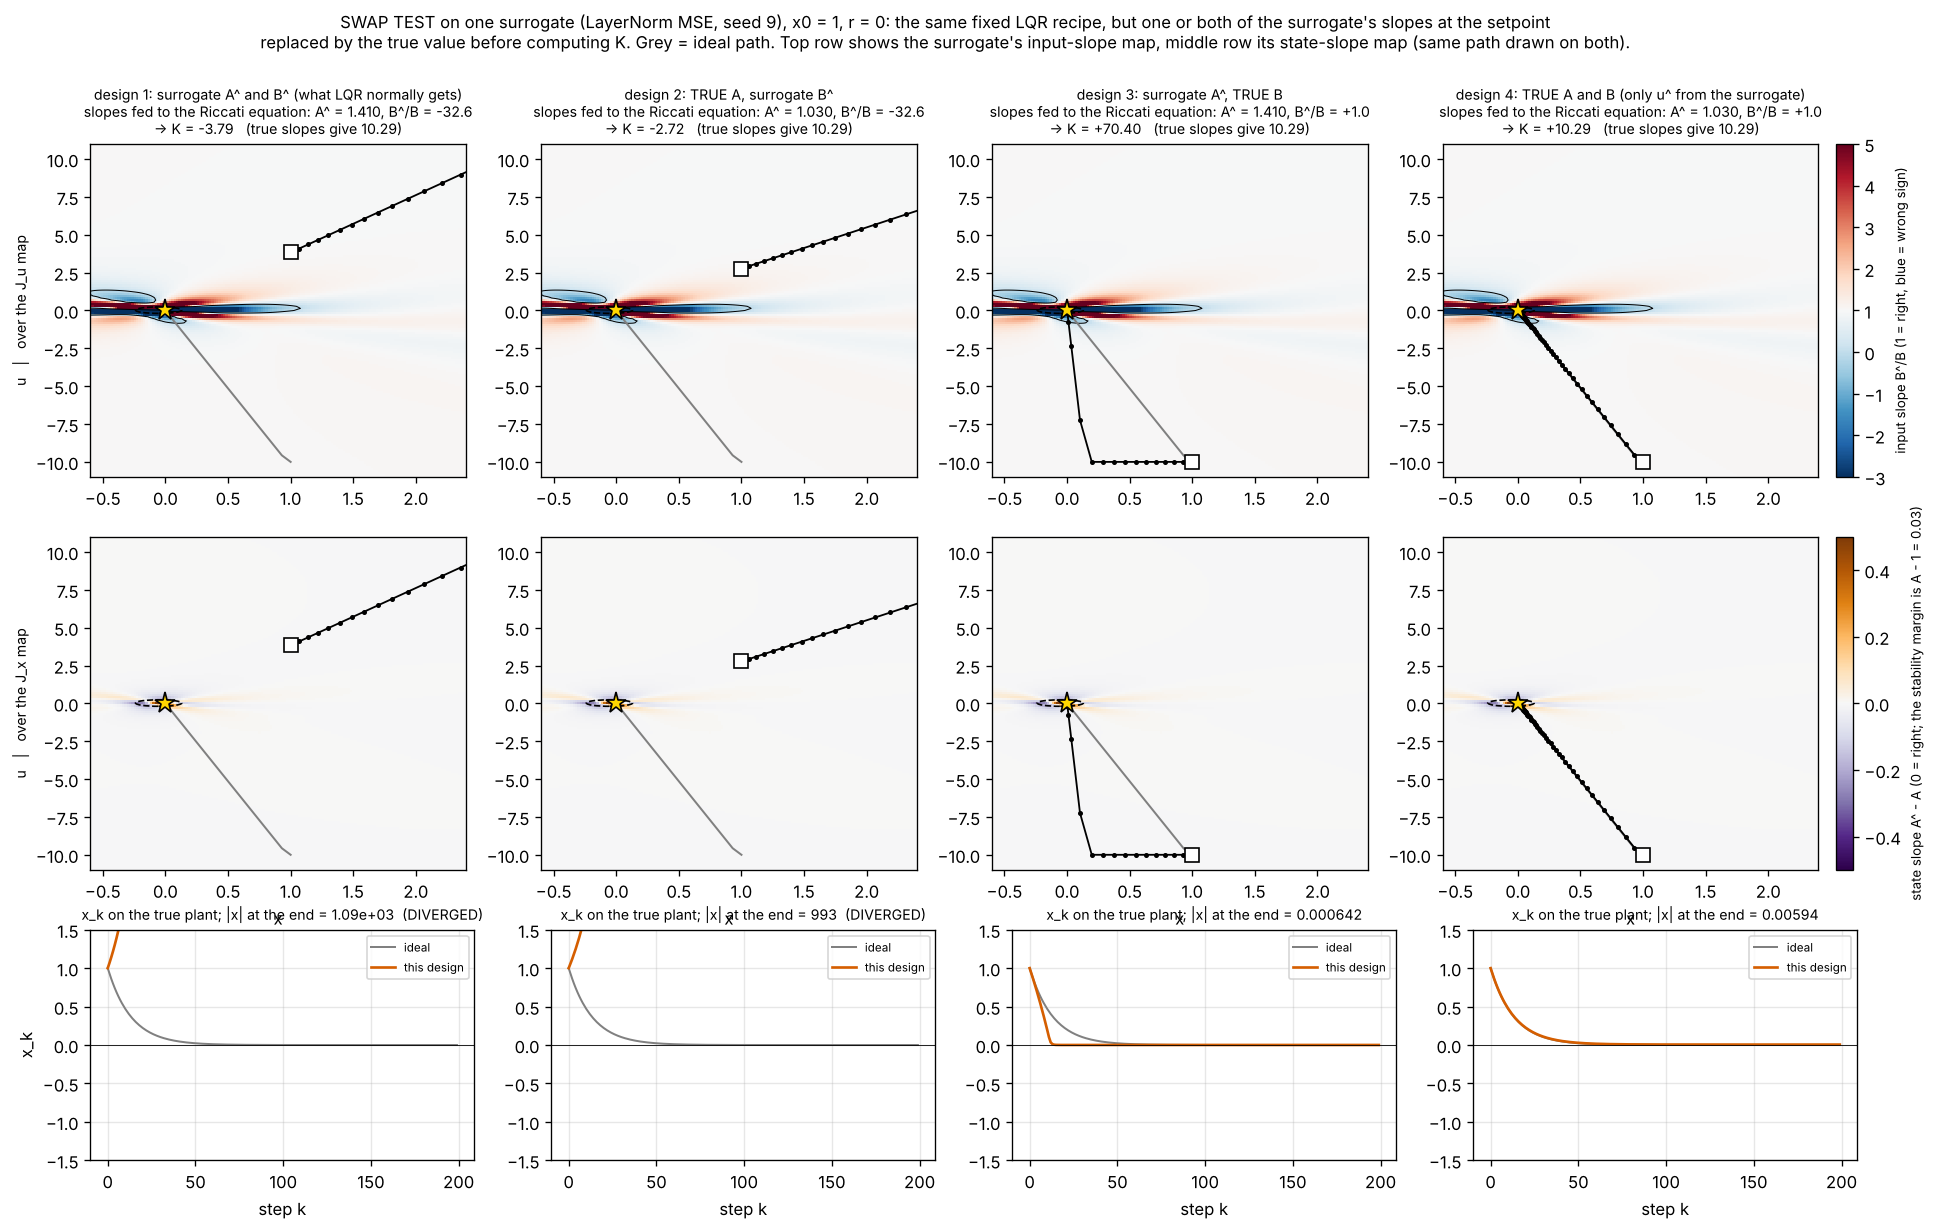
\includegraphics[width=\textwidth]{f13_swap_seed9.png}
\caption{Swap test on LN MSE 3000, seed 9, $x_0=1$, $r=0$. Columns: designs 1 to 4 (title: the slopes fed to the Riccati equation and the resulting $K$). Top: path over the $\hat J_u/B$ map. Middle: the same path over the $\hat J_x-A$ map. Bottom: $x_k$ (orange) against the ideal (grey). Designs 1 ($K=-3.79$) and 2 ($K=-2.72$) diverge because the input slope has the wrong sign; design 3 ($K=+70.4$, true $B$ but $\hat A=1.41$) is very aggressive, saturates at $-10$, and still converges from this start; design 4 ($K=10.29$) follows the ideal path up to an offset of 0.006.}
\label{fig:swap9}
\end{figure}

\begin{figure}[H]
\centering
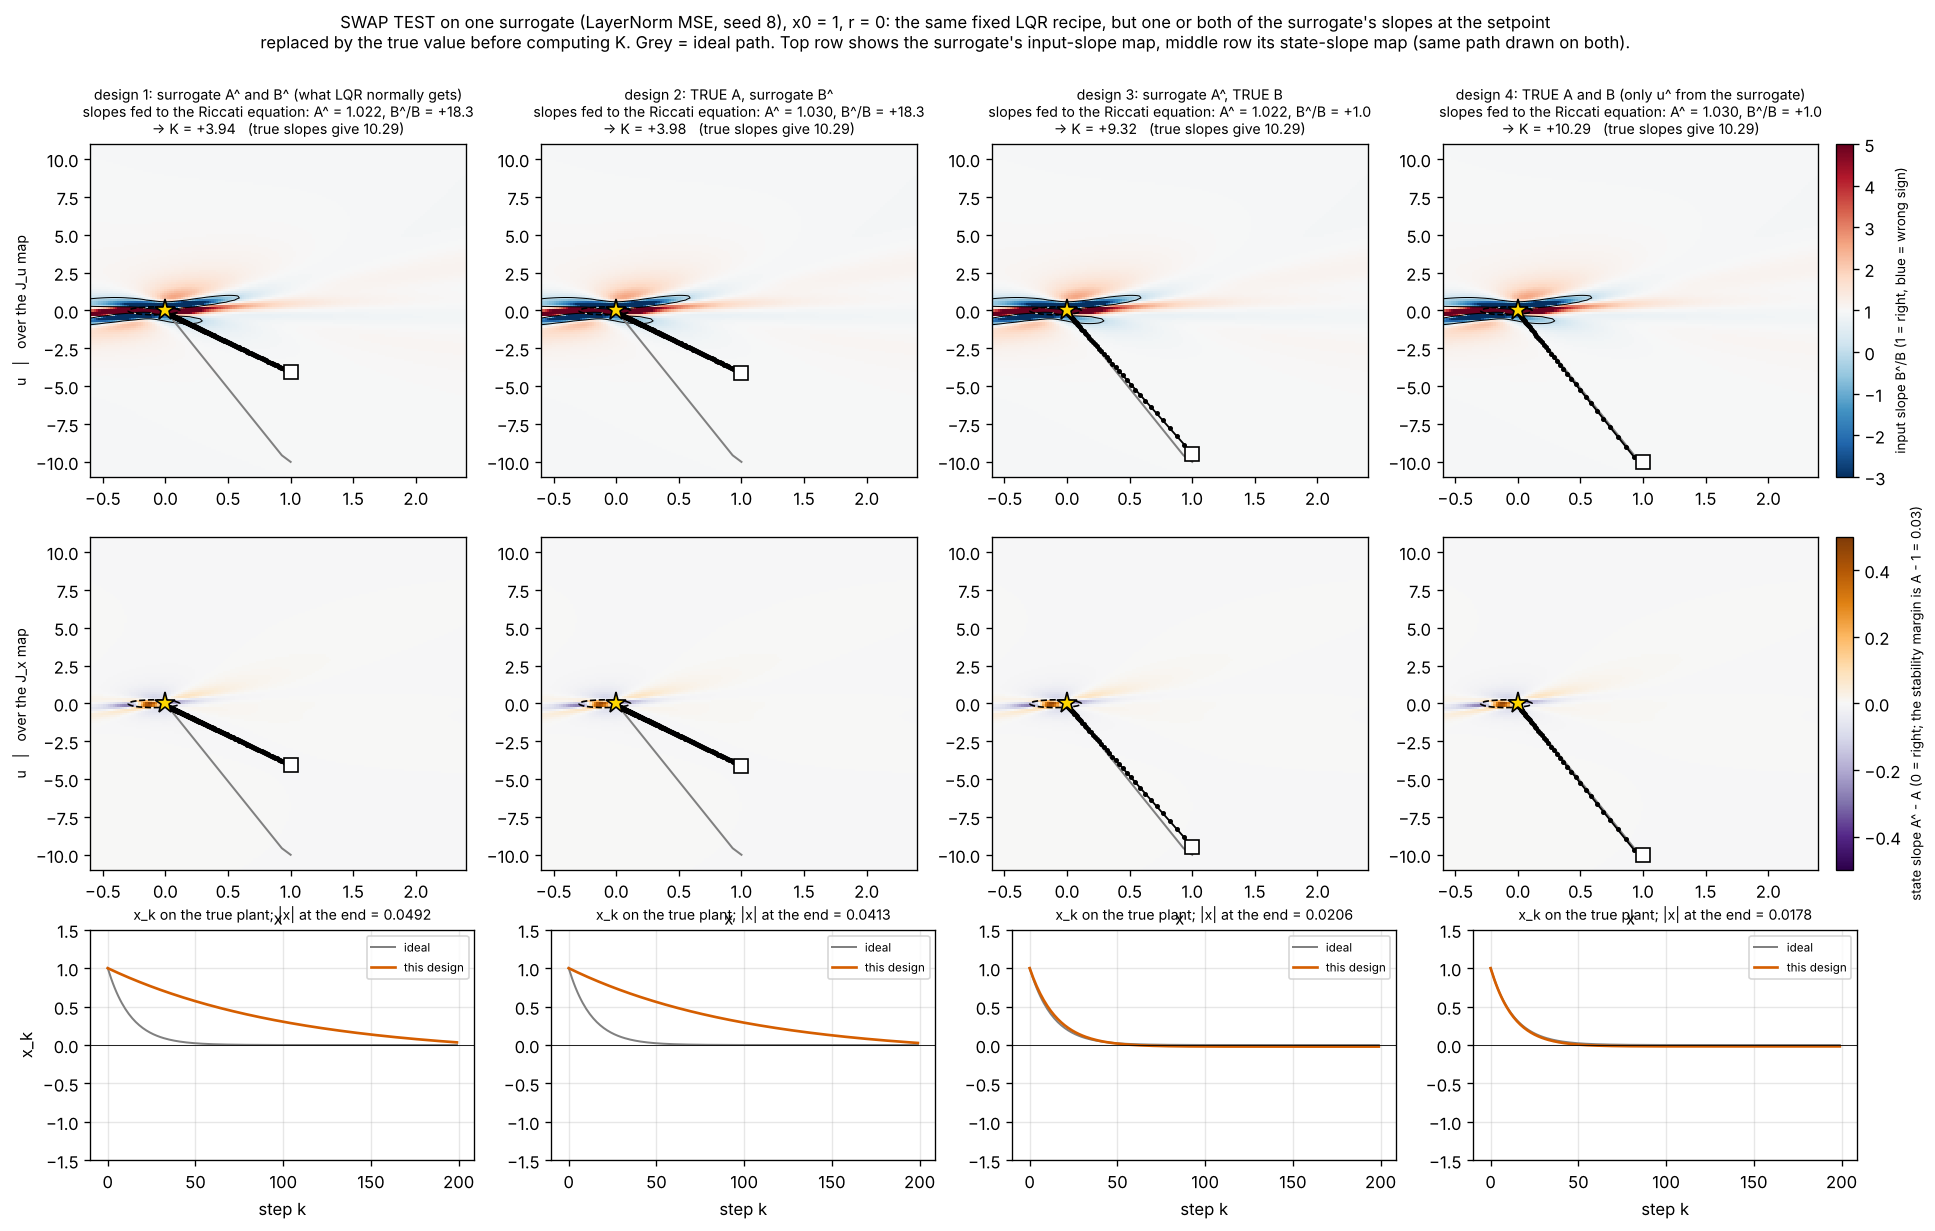
\includegraphics[width=\textwidth]{f14_swap_seed8.png}
\caption{The same for seed 8 (overestimated input slope at the setpoint, $\hat B/B=18.3$, $\hat A=1.022$). Designs 1 and 2 give $K=3.94$ and $3.98$: slow convergence ($x_{200}=0.033$ and $0.025$). Design 3 gives $K=9.32$ and design 4 $K=10.29$: both close to the ideal.}
\label{fig:swap8}
\end{figure}

\begin{figure}[H]
\centering
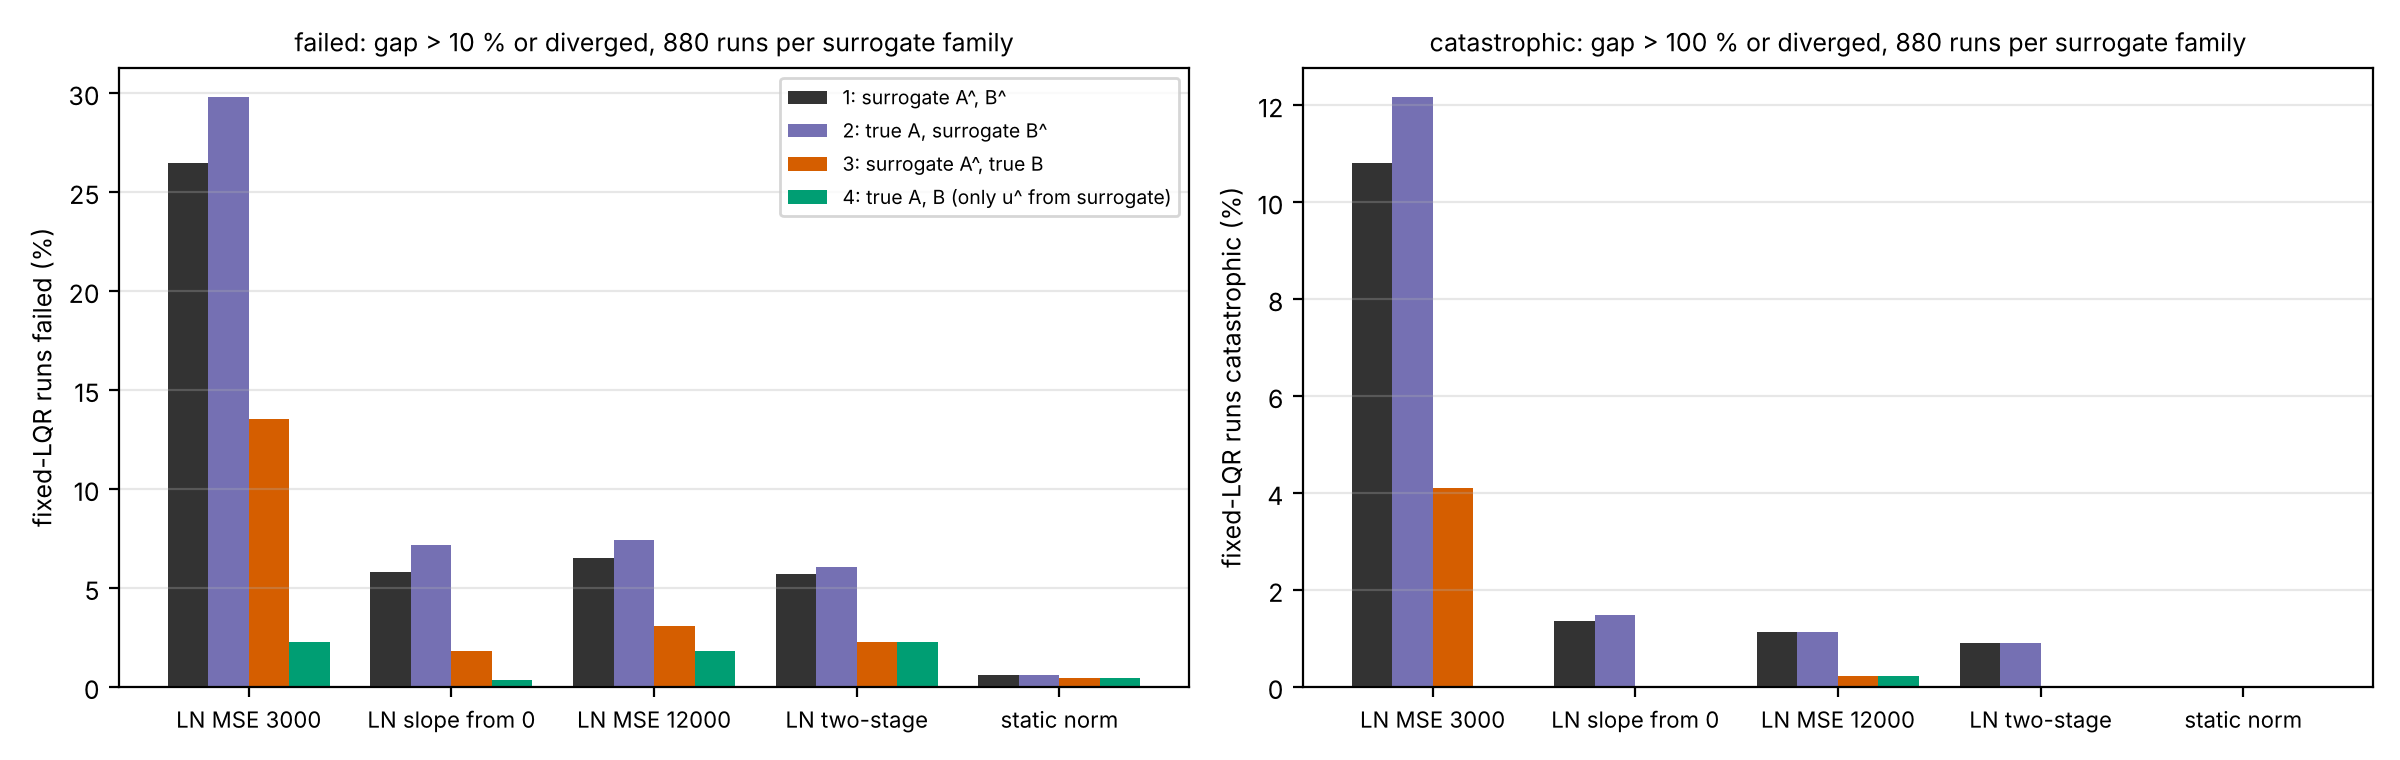
\includegraphics[width=\textwidth]{f15_swap_rates.png}
\caption{Swap test over the whole grid: fixed-LQR failure (left) and catastrophic (right) rates for the four designs and five surrogate families, 880 runs each.}
\label{fig:swaprates}
\end{figure}

\subsection{Numbers}
\begin{center}
\begin{tabular}{lcccc}
\toprule
LN MSE 3000, fixed LQR & $\hat A$ & $\hat B$ & failed (\%) & catastrophic (\%) \\
\midrule
Design 1 (what LQR normally gets) & surrogate & surrogate & 26.5 & 10.8 \\
Design 2 & true & surrogate & 29.8 & 12.2 \\
Design 3 & surrogate & true & 13.5 & 4.1 \\
Design 4 (only $\hat u$ from the surrogate) & true & true & 2.3 & 0.0 \\
\bottomrule
\end{tabular}
\end{center}
Design 1 to design 4, other families: LN slope from step 0 5.8 to 0.3; LN MSE 12000 6.5 to 1.8; LN two-stage 5.7 to 2.3; static norm 0.6 to 0.5 percent failed. Setpoint slope errors of LN MSE 3000 over the 110 seed-setpoint designs: $|\hat A-A|$ median 0.007, maximum 0.50; $|\hat B/B-1|$ median 0.34, maximum 87 (seed 2, $r=0$).

\subsection{Why a tiny $\hat A$ error matters: the stability margin}
With the true $B$, the gain depends strongly on $\hat A$ near $A=1.03$. For $x_0=1$, $r=0$ and $\hat u=0$:
\begin{center}
\begin{tabular}{rrrr}
\toprule
$\hat A$ & $K=\mathrm{DARE}(\hat A,B)$ & true pole $1.03-0.01K$ & gap \\
\midrule
0.90 & 2.10 & 1.009 & +11\,191 \% (still growing) \\
0.95 & 3.50 & 0.995 & +393 \% \\
0.98 & 5.15 & 0.978 & +62 \% \\
1.00 & 6.83 & 0.962 & +16 \% \\
1.03 & 10.29 & 0.927 & 0 \\
1.10 & 21.02 & 0.820 & +12 \% \\
1.41 & 70.43 & 0.326 & +27 \% \\
\bottomrule
\end{tabular}
\end{center}
An $\hat A$ error of only $-0.03$ (the model believes the plant is marginally stable) already fails the 10 percent threshold, and $-0.08$ to $-0.13$ is catastrophic. Overestimates give aggressive gains that saturate and cost 10 to 30 percent more but rarely diverge. Errors of 0.03 to 0.5 occur near the kink, i.e. 1 to 17 times the margin $A-1$.

\subsection{Hypothesis, observation, conclusion}
Hypothesis H3: the $\hat J_u$ kink is the main cause of the LQR failures (with low authority a wrong-signed $\hat B$ flips the sign of $K$, and an overestimated $\hat B$ lowers $K$ towards the stability limit $K=3$); $\hat J_x$ is secondary.

Observations.
\begin{itemize}
\item Making $B$ true (design 3) halves the failures (26.5 to 13.5 percent) and removes most catastrophes (10.8 to 4.1).
\item Making $A$ true alone (design 2) removes nothing; the rates even rise slightly (29.8 and 12.2), because on some seeds the two errors pushed $K$ in opposite directions and partly cancelled inside the Riccati equation. The effects are not additive ($26.5<29.8+13.5$), which is why attribution must be done by swapping, not by summing.
\item Making both true (design 4) leaves 2.3 percent mild failures and no catastrophes: the remaining failures are the steady offsets caused by the value error in $\hat u$, present at the same level in the two-stage family (2.3 percent).
\end{itemize}
Conclusion. For LQR both slopes matter. The input slope carries all of the damage that cannot be removed by fixing the other slope, and the state slope alone still causes 13.5 percent failures and 4.1 percent catastrophes despite its small absolute error, because the LQR gain depends on $\hat A-1$, the unstable part, whose true value is only 0.03. The value error is not the cause of the catastrophic failures. (For DPC, slide 20, the same swap applied inside backpropagation shows that the gradient explosion disappears with the true $\hat J_u$ and is unchanged with the true $\hat J_x$.)

Why it matters. This is causal evidence (an intervention), not a correlation, and it says which derivative a slope check or a slope loss must get right.

%=====================================================================
\section{Summary of conclusions up to slide 14, limits, and corrections}\label{sec:summary}

\begin{enumerate}
\item H0 is false for LayerNorm surrogates: the same value accuracy gives 26.5 percent fixed-LQR failures (10.8 catastrophic) against 0.6 (0) for a static-norm surrogate.
\item The defect is structural and located: an ellipse around $z^\star$ whose half-widths $D/\|q_x\|$ and $D/\|q_u\|$ follow from the encoder weights and the bias residual $c_\perp$, with alternating-sign petals that decay algebraically ($1/d$ along the setpoint line).
\item When a controller reads the slopes decides where the kink hurts: once at the setpoint for the fixed LQR (damage set by the setpoint's distance from the kink, about $0.5/d$), along the path for the rescheduled LQR (damage set by the petals the path crosses).
\item Both slopes matter for LQR; $\hat J_u$ dominates, and $\hat J_x$ matters through the small stability margin $A-1$.
\end{enumerate}

Limits.
\begin{itemize}
\item One scalar linear plant with $A=1.03$, $B=0.01$. The mechanism is dimension-free; the failure rates are specific to this plant.
\item One architecture (pre-norm, $H=16$). Other normalisations are predictions.
\item The 10 percent threshold also catches value-error offsets; the catastrophic rate is the measure that is unambiguously the kink.
\item The kink ellipse drawn in the figures is axis-aligned; the exact one is tilted by a modest amount.
\item The petal decay is $1/d$ along the setpoint direction but faster for the largest error on a circle at intermediate distances (Figure~\ref{fig:petals}).
\end{itemize}

Corrections to the presentation briefing made in this document.
\begin{itemize}
\item The surrogate is $\hat F=w_d^\top(h+g)+b_d$ with the residual connection in the 16-dimensional latent space, not $[x,u]+\dots$ (Section~\ref{sec:net}).
\item Slope labels for two-stage and slope-from-step-0 are estimated from the data, not the true slopes (Section~\ref{sec:labels}).
\item The maximum setpoint input-slope error of 87 times $B$ is seed 2 at $r=0$; seed 9's setpoint value is $-32.6$. The largest error anywhere in the box is 200.9 (seed 2).
\item The kink width is set by $\|c_\perp\|$, not by $\epsilon$ (Section~\ref{sec:kink}).
\item Seed 8's fixed-LQR loop has pole 0.991 (slow but stable), not 1.00.
\item Rescheduled-LQR catastrophic rate for LN MSE 3000 is 3.4 percent against the true LQR oracle (the 3.6 percent in the notes was measured against the tracking-DPC oracle).
\item The far-field decay is $1/d$ along the setpoint line; the maximum over directions decays faster at $d=2$ to 20.
\end{itemize}

%=====================================================================
\section{Reproducing everything}\label{sec:repro}

\subsection{Code}
\begin{itemize}
\item level1\_core.py (project folder claude/dpc/): plant, data, label estimator, network, losses, trainer, kink geometry, DARE.
\item dpc\_core.py: surrogate training driver (train\_surrogates), DPC controllers and evaluation.
\item phase\_core.py: surrogate equilibrium, fixed and rescheduled LQR, metrics (track\_metrics, seen\_gain, kink\_visits), the LQR study (lqr\_study), tracking DPC.
\item Notebooks: dpc\_through\_surrogates.ipynb (trains and saves the six surrogate families, 10 seeds, and the regulation DPC controllers) and dpc\_phase\_tracking.ipynb (LQR study and tracking DPC), built by build\_dpc\_notebook.py and build\_phase\_notebook.py.
\item For this document: run\_lqr\_study.py (runs the LQR study on the saved surrogates and writes lqr\_study.csv; 30 s on a CPU) and make\_figs.py (all figures except Figures~\ref{fig:four}, \ref{fig:resched}, \ref{fig:surf3d}, \ref{fig:swap9}, \ref{fig:swap8} and all numbers quoted here; 20 s on a CPU). Figures~\ref{fig:four} and \ref{fig:resched} come from story/lqr\_story.py, Figures~\ref{fig:swap9} and \ref{fig:swap8} from story/swap\_story.py, Figure~\ref{fig:surf3d} from make\_fig3d.py (10 s on a CPU), and the swap rates from story/attribution.py.
\end{itemize}

\subsection{Steps}
\begin{enumerate}
\item Train the surrogates: run dpc\_through\_surrogates.ipynb with SEEDS = range(10), SIGMA = 0.01, KERNEL = ``epan'' and the plant Plant(A=1.03, B=0.01, eps\_nl=0). Surrogates are saved to dpc\_out/surrogates/<name>.npz (weights, static-norm scales, metrics). Each family trains in seconds to a few minutes on a GPU; the slope families also compute the labels once.
\item Run run\_lqr\_study.py, then make\_figs.py, pointing OUT to the folder with surrogates/.
\item For the swap test, run story/attribution.py (rates) and story/swap\_story.py (figures).
\end{enumerate}
Software used for the numbers here: Python 3.13, JAX 0.12 (float64 enabled), NumPy 2.5, SciPy 1.18, optax 0.2.8, pandas 3.0, Matplotlib 3.11. The saved surrogates reproduce the earlier Kaggle numbers to every printed digit (seed 0 of LN MSE 3000: $\max|\hat J_u/B-1|=11.3558$, rel-MSE $1.2545\times10^{-6}$), and the LQR study run locally and on Colab agree (median relative cost difference $4\times10^{-16}$).

%=====================================================================
\appendix
\section{Key functions}

The network, the normalisation and the data (level1\_core.py):
\begin{lstlisting}[language=Python]
XMAX, UMAX = 4.0, 10.0          # data box
N_DATA, N_TEST = 20000, 4000
H, WB, EPS = 16, 32, 1e-6       # encoder width, branch width, LayerNorm epsilon
LR = 3e-3                       # Adam, full batch
LQR_Q, LQR_R = 5.0, 0.1

def make_data(plant, sigma, data_seed, n=N_DATA):
    rng = np.random.default_rng(data_seed)
    x = rng.uniform(-XMAX, XMAX, n)
    u = rng.uniform(-UMAX, UMAX, n)
    y = plant.f(x, u) + sigma * rng.standard_normal(n)
    return dict(x=x, u=u, y=y)

def init_params(seed):
    k = jax.random.split(jax.random.PRNGKey(int(seed)), 4)
    kb = jax.random.split(k[2], 8)
    return dict(E=_glorot(k[0], (2, H)), b=jnp.zeros(H), gamma=jnp.ones(H), beta=jnp.zeros(H),
                Wd=_glorot(k[1], (H, 1)), bd=jnp.zeros(1),
                br=dict(W1=_glorot(kb[0], (H, WB)), b1=jnp.zeros(WB),
                        W2=_glorot(kb[1], (WB, H)), b2=jnp.zeros(H)))

def _norm(kind, h, s0):
    if kind == "none":
        return h
    r = h - jnp.mean(h, -1, keepdims=True)
    if kind == "layer":
        return r / jnp.sqrt(jnp.mean(r ** 2, -1, keepdims=True) + EPS)
    if kind == "static":
        return r / s0

def F_point(p, x, u, s0, norm):
    h = x * p["E"][0] + u * p["E"][1] + p["b"]
    v = _norm(norm, h, s0)
    a = jax.nn.gelu((p["gamma"] * v + p["beta"]) @ p["br"]["W1"] + p["br"]["b1"], approximate=False)
    return h @ p["Wd"][:, 0] + (a @ p["br"]["W2"] + p["br"]["b2"]) @ p["Wd"][:, 0] + p["bd"][0]
\end{lstlisting}

The loss (level1\_core.py, make\_loss): kind "mse" or "sob" (value plus slope):
\begin{lstlisting}[language=Python]
def loss(p, key, D, wx, wu, lam):
    mse = jnp.mean((Fb(p, D["x"], D["u"], D["s0"]) - D["y"]) ** 2)
    if kind == "mse":
        return mse
    idx = ...  # M = 2048 indices drawn uniformly with replacement
    jx, ju = _derivs(Fb, p, D["x"][idx], D["u"][idx], D["s0"])   # jax.jvp
    reg = jnp.mean(wx * D["sx"] ** 2 * (jx - D["Jx_lab"][idx]) ** 2
                   + wu * D["su"] ** 2 * (ju - D["Ju_lab"][idx]) ** 2)
    return mse + lam * reg
\end{lstlisting}

Kink geometry and the Riccati gain (level1\_core.py):
\begin{lstlisting}[language=Python]
_PM = np.eye(H) - np.ones((H, H)) / H

def kink_center(p):
    E, b = np.asarray(p["E"], float), np.asarray(p["b"], float)
    A = _PM @ E.T                                       # Q_E = P E (E is stored transposed)
    c0 = _PM @ b                                        # c = P b
    z = -np.linalg.lstsq(A, c0, rcond=None)[0]          # z* = (x*, u*)
    r = A @ z + c0                                      # c_perp
    D = np.sqrt(r @ r + H * EPS)                        # D = sqrt(H) delta
    return z, D / np.linalg.norm(A[:, 0]), D / np.linalg.norm(A[:, 1])   # z*, r*_x, r*_u

def dare_K(a, b, Q=LQR_Q, R=LQR_R):
    b2 = b * b
    coef = R - Q * b2 - a * a * R
    P = np.where(b2 > 1e-14, (-coef + np.sqrt(coef ** 2 + 4 * b2 * Q * R)) / (2 * b2), np.nan)
    return np.where(b2 > 1e-14, a * b * P / (R + b2 * P), 0.0)
\end{lstlisting}

The LQR closed loops (phase\_core.py):
\begin{lstlisting}[language=Python]
def run_lqr(design, plant_model, r, x0, kind, N=200):
    uh, nroot, ah, bh = equilibrium(design, r)          # u_hat(r) and slopes at (r, u_hat)
    Kf = L.dare_K(ah, bh)
    x, u_prev = np.asarray(x0, float).copy(), uh.copy()
    xs, us, Ks = [x], [], []
    for _ in range(N):
        if kind == "fixed":
            K = Kf
        else:                                           # rescheduled
            _, a, b = design.fj(x, u_prev)              # slopes at (x_k, u_{k-1})
            K = L.dare_K(a, b)
        u = np.clip(uh - K * (x - r), -10, 10)
        x = plant_model.plant.f(x, u)                   # the TRUE plant
        xs.append(x); us.append(u); Ks.append(K)
        u_prev = u
    return np.stack(xs), np.stack(us), np.stack(Ks), dict(uh=uh, nroot=nroot, ah=ah, bh=bh, K_fixed=Kf)

def track_cost(xs, us, r, plant):
    uss = plant.u_ss(r)
    return (Q * (xs[:-1] - r) ** 2 + R * (us - uss) ** 2).sum(0) + QF * (xs[-1] - r) ** 2

def track_metrics(xs, us, r, plant, ref_cost=None):
    J = track_cost(xs, us, r, plant)
    fin = np.abs(xs[-20:].mean(0) - r)                  # offset
    div = ~np.isfinite(xs).all(0) | (np.nanmax(np.abs(xs), 0) > 10.0)
    out = dict(cost=J, offset=fin, diverged=div)
    if ref_cost is not None:
        out["gap"] = J / ref_cost - 1.0
    return out
\end{lstlisting}

The swap test (story/attribution.py):
\begin{lstlisting}[language=Python]
uh, nroot, ah, bh = PC.equilibrium(m, r)
designs = [("both from surrogate", L.dare_K(ah, bh)),
           ("true A, surrogate B", L.dare_K(np.full_like(ah, A), bh)),
           ("surrogate A, true B", L.dare_K(ah, np.full_like(bh, B))),
           ("both true",           L.dare_K(np.full_like(ah, A), np.full_like(bh, B)))]
for tag, K in designs:
    xs, us = sim(uh, K)                 # u = clip(uh - K (x - r), +-10) on the true plant, 200 steps
    met = PC.track_metrics(xs, us, r, plant, J_oracle)
    far = np.abs(x0 - r) >= 0.5
    failed = (met["diverged"] | (met["gap"] > 0.1))[far].mean()
    catastrophic = (met["diverged"] | (met["gap"] > 1.0))[far].mean()
\end{lstlisting}

\end{document}
